%File: formatting-instruction.tex
\documentclass[letterpaper]{article} %DO NOT CHANGE THIS
\usepackage{aaai19}  %Required
\usepackage{times}  %Required
\usepackage{helvet}  %Required
\usepackage{courier}  %Required
\usepackage{url}  %Required
\usepackage{graphicx}  %Required
\usepackage{amsmath}
\usepackage{mathrsfs}
\usepackage{color,soul}
\usepackage{listings}
\usepackage{caption,subcaption}
\usepackage{natbib}
\usepackage{multirow}
\usepackage{hhline}
\usepackage{mathrsfs}  
\usepackage{amsfonts}  
\usepackage{amsthm}
\usepackage{comment}




\newtheorem{mydef}{Definition}
\newtheorem{define}{Definition}
\newtheorem{prop}{Proposition}

\newcounter{tmp}

% \usepackage{fontspec}
% \usepackage{unicode-math}
% \newcommand{\stripsp}{{\sc strips+}}
\newcommand{\stripsp}{{\sc STRIPS+}}
% \newcommand{\pddlthree}{{\sc PDDL3}}
\newcommand{\pddlthree}{{PDDL3}}
\newcommand{{\lama}}{{{LAMA}}}
\newcommand{\mercury}{{Mercury}}
\newcommand{{\fdss}}{{Fast Downward Stone Soup 2018}}
\newcommand{{\fdssshort}}{{FDSS 2018}}
\newcommand{\lamapruning}{$\text{LAMA}_{\text{P}}(h_\text{R})$}

\newcommand{{\miplan}}{{MIPlan}}
\newcommand{{\ibacop}}{{IBaCoP2}}
\newcommand{{\fdremixcomplete}}{{Fast Downward Remix}}
\newcommand{\lprpgp}{{LPRPG-P}}
\newcommand{{\fdremix}}{{FDRemix}}
% \newcommand{{\fifthIPC}}{{{IPC5}}}

\newcommand{\strips}{{\sc strips}}
\newcommand{\adl}{{\sc adl}}
\newcommand{\pddlIII}{{\sc{pddl3}}}
\newcommand{\stripspap}{{\sc strips+ap}}
\newcommand{\stripspp}{{\sc strips+p}}
\newcommand{\pddl}{{\sc pddl}}
% new command
\newcommand{\hplanp}{{HPlan-P}}
\newcommand{\mipsxxl}{{MIPS-XXL}}
\newcommand{\lpg}{{LPG}}
\newcommand{{\GBLcoles}}{{{GBL15-NB-B15}}}
% \newcommand{{\fifthIPC}}{{ {IPC5}}}
% \newcommand{{\fifthIPC}}{{\footnotesize {IPC5}}}
\newcommand{{\fifthIPC}}{{{IPC5}}}
\newcommand{\threatA}{T_{\mathcal{A}}(o)}
\newcommand{\violA}{V_{\mathcal{A}}(o)}
\newcommand{\threatSB}{T_{\mathcal{SB}}(o)}
\newcommand{\supportSB}{S_{\mathcal{SB}}(o)}
\newcommand{\threatAMO}{T_{\mathcal{AO}}(o)}
\newcommand{\supportST}{S_{\mathcal{ST}}(o)}
\newcommand{\affected}{\mathcal{I}(o)}
\newcommand{\truettt}{\small \texttt{TRUE}}
\newcommand{\pviol}{P\textit{-violated}}
\newcommand{\affectedd}{P_{\textit{affected}}(o)}
\newcommand{\lamap}{
$\text{LAMA}_{\text{P}}(h_{\text{R}}$}


\frenchspacing  %Required
\setlength{\pdfpagewidth}{8.5in}  %Required
\setlength{\pdfpageheight}{11in}  %Required
%PDF Info Is Required:
  \pdfinfo{
/Title (On Compiling PDDL3 Qualitative Preferences without Using Automata)
/Author (Anonymous)}
\setcounter{secnumdepth}{0}  
 \begin{document}
% The file aaai.sty is the style file for AAAI Press 
% proceedings, working notes, and technical reports.
%
\title{On Compiling Away PDDL3 Soft Trajectory Constraints without Using Automata}
%\title{On Compiling Away PDDL3 Qualitative Preferences without Using Automata}
\author{...
}
\maketitle
\begin{abstract}
We address the problem of propositional planning extended with the class of soft temporally extended goals supported in {\pddlIII}, also called qualitative preferences since IPC-5.
%that is part of the standard planning language 
% {\pddl} since the 5th International Planning Competition (\fifthIPC). 
Such preferences are useful to characterise plan quality by allowing the user to express certain soft constraints on the state trajectory of the desired solution plans.
We propose and evaluate a compilation approach that 
extends previous work on compiling soft reachability goals and always goals to the full set of {\pddlIII} qualitative preferences.
This approach directly compiles qualitative preferences into propositional planning without using automata to represent the trajectory constraints. Moreover, since no numerical fluent is used, it allows 
many existing {\strips} planners to immediately address planning with preferences. 

%While other existing approaches represent {\pddlIII} soft state-trajectory constraints as particular automata that are compiled into a planning problem with numerical fluents, our approach directly compile them into propositional planning with action costs. 

%Our compilation extends previous work that was limited to soft reachability goals and state-invariant (always) goals to the full set of {\pddlIII} qualitative preferences.
%
%Starting from the work of Keyder and Geffner on compiling (reachability)
%soft goals, we propose a compilation scheme
%for translating a {\strips} problem enriched with qualitative  {\pddlIII}
%preferences  (and possibly also with soft goals) into an equivalent {\strips}
%problem with action costs. 
%The proposed compilation, which supports all types of qualitative preferences in the benchmarks
%from \fifthIPC, allows many existing {\strips} planners to immediately address
%planning with preferences. 
An experimental analysis presented in the paper evaluates the performance of
state-of-the-art propositional planners supporting action costs using our compilation
%approach to deal with 
of
{\pddlIII} qualitative   preferences.  The results indicate
that our approach is highly competitive with respect to current planners that
natively support the considered class of preference, as well as with a recent automata-based compilation approach.
\end{abstract}



%%%%%%%%%%%%%%%%
% INTRODUZIONE %
%%%%%%%%%%%%%%%%
\section{Introduction}
Planning with preferences, also called ``over-subscription planning" in \cite{Briel-et-al:AAAI04,do-kambhampati04,smith04}, concerns the generation of plans for problems involving soft goals or soft state-trajectory constraints (called preferences in \pddlIII), that it is desired a plan satisfies, but that do not have to be satisfied. The quality of a solution plan for these problems depends on the soft goals and preferences that are satisfied.

For instance, a useful class of preferences than can be expressed in {\pddlIII} \cite{GHLS+09} consists of  {\em always preferences}, requiring that a certain condition should hold in {\em every} state reached by a plan. As discussed in \cite{Weld:94AA,bacKab,GHLS+09,Hplanp:aij09}, adding always preferences to the problem model can be very useful to express safety or maintenance conditions, and other desired plan properties. An simple example of such conditions is ``whenever a building surveillance robot is outside a room, all the room doors should be closed". 

{\pddlIII} supports other useful types of preferences, and in particular the qualitative preferences of types {\em at-end}, which are which are equivalent to soft goals, {\em sometime}, {\em sometime-before} and  {\em at-most-once}, which are all the types used in the available benchmarks for planning with qualitative {\pddlIII} preferences \cite{GHLS+09}. Examples of preferences that can be expressed  through these constructs in a logistics domain are: ``sometime during the plan the fuel in the tank of every vehicle should be full'', ``a certain depots should be visited before another once'',  ``every store should be visited at most once'' (the reader can find additional examples in \cite{GHLS+09}).
 
In this paper, we study propositional planning with these types of preferences through a compilation approach. 




%%%%%%%%%%%%%%%%
% RELATED WORK %
%%%%%%%%%%%%%%%%
\section{Related Work}
Our compilative approach is inspired by the work of Keyder and Geffner \cite{kn:geffner09}
on compiling soft goals into {\strips} with action costs (here denoted with \stripsp). In this work
the compilation scheme introduces, for each soft goal $p$ of the problem, a dummy goal $p'$ that
can be achieved using two actions in mutual exclusion. The first one, which is called \textit{collect(p)},
has cost equal to 0 and requires that $p$ be true when it is applied; the second one, whic is called \textit{forgo(p)},
has cost equal to the utlity of $p$ and requires that $p$ be false when it is applied.
\\\indent Both of these action can be performed at the end of the plan and for each soft goal $p$ but just one of
$\{$\textit{collect(p), forgo(p)}$\}$ can appear in the plan depending on whether the soft goal
has been achived or not. This scheme has achieved good perfomance which can be improved with the use of
an ad hoc admissible heuristic based on the reachability of soft goals \cite{percassi2017improving}.

The most prominent existing planners supporting {\pddlIII} preferences are {\hplanp} \cite{Hplanp:aij09,BM:AAAI06},
which won the ``qualitative preference" track of IPC-5, {\mipsxxl} \cite{edelkamp2006compilation,edelkamp2006large}
and the more recent {\lprpgp} \cite{coles2011lprpg}
and its extension in \cite{coles2013searching}.
%
These (forward) planners represent preferences through automata whose states are synchronised with the states generated by the action plans, so that an accepting automaton state corresponds to preference satisfaction. For the synchronisation, {\hplanp} and {\lprpgp} use planner-specific techniques, while {\mipsxxl} compiles the automata by modifying the domain operators and adding new ones modelling the automata transitions of the grounded preferences. 

Our computation method is very different from the one of {\mipsxxl} since, rather than translating automata into new operators, the problem preferences are compiled by only modifying the domain operators, possibly creating multiple variants of them. Moreover, our compiled files only use {\stripsp}, while {\mipsxxl} also uses numerical fluents.\footnote{Another compilation scheme using numerical fluents is considered in \cite{GHLS+09} to study the expressiveness of \pddlIII (without an implementation).}

The works on compiling LTL goal formulas by Cresswell and Coddington \cite{CC:ECAI04} and Rintanen \cite{Rintanen:ECAI00}
are also somewhat related to ours, but with important differences. Their methods handle {\em hard} temporally extended
goals instead of preferences, i.e., every temporally extended goal must be satisfied in a valid plan, and hence there
is no notion of plan quality referred to the amount of satisfied preferences. Rintanen's compilation considers only
single literals in the always formulae (while we deal with arbitrary CNF formulas), and it appears that extending
it to handle more general formulas requires substantial new techniques \cite{Rintanen:personal2015}. 
An implementation of Crosswell and Coddington's approach is unavailable, but Bayer and McIlaraith \cite{BM:AAAI06} observed
that their approach suffers exponential blow up problems and performs less efficiently than the approach of {\hplanp}.

\hl{IMPORTANTE, CONFRONTO LAVORO NEBEL:} An important work about soft-trajectory constraints compilation,
which is closely related to ours, has been recently proposed by Wright, Matt\"uller and
Nebel in \cite{nebel2018} (cerca riferimento articolo Nebel). This approach is a based
on the compilation of the soft trajectory constraints into conditional effects and state dependent action costs using
$\sf{LTL}_{\text{f}}$ and B{\"u}chi automata. There are some similarities between  
between our and their approach but at the same time there are also
differences. 

\textbf{FP: differenze approccio Nebel e nostro: 1) numero di fluenti introdotto nella compilazione diverso; 2) il nostro
e' un approccio piu' specifico PDDL3-oriented, il loro piu' generale; 3) diverso meccanismo di aggiornamento dei costi, nel loro caso
ricompensa e penalita', nel nosto solo penalità 4) il loro schema prevede quindi costi negativi e postivi, il nostro positivi; nel loro caso per avere solo costi positivi e' necessario perdere l'ottimalita' nel nostro caso no ed inoltre volendo potremmo introdurre dei costi
negativi per quelle preferenze la cui violazione puo' essere testata solo alla fine del piano mantenendo l'ottimalita'; ho fatto inoltre menzione del fatto che i costi possono essere incrementanti il prima possibile (es. always)}

\textbf{1)} In our approach, given a preference $P$,
we introduce at most a pair of boolean fluents, typically one additional fluent to 
represent if a preference is violated or not ($P\textit{-violated}$) and
in some cases an additional fluent to correctly represent the status of a preference during
the planning,
while in their approach it is introduced a boolean variable
for each state of the corresponding automaton of $P$. \textbf{2)} Their approach is more general
while ours is focused on PDDL3 constraints and therefore it is more specific.

\textbf{3)} In their work the cost of the plan during the planning is updated by using rewards
and penalties (negative and positive costs respectively). The cost of the plan is increased whenever
a violation of a preference (also reversible) occurs. On the contrary,
if an operator causes the satisfaction of a preference then the cost of the plan is decreased.
In both cases the negative or positive cost is equal to the utility of the interested preference\footnote{
\hl{Messo in footnote altrimenti era troppo lungo:}
Note that 
both the violation and the satisfaction of a preference may be temporary conditions depending on the type 
of interested preference. For example an always preference can be irreversibly violated and its satisfaction can only be evaluated at the end of the plan considering the whole trajectory of the states; on the contrary a sometime-after preference can be satisfied and violated several times during the execution of the plan.
}. \textbf{4)} This type of cost update requires the use of negative costs while our compilation scheme produces a problem
whose costs are monotonically increasing because, similarly to what was proposed in Keyder and Geffner,
costs are realized only at the end of the planning. In our scheme some costs can be anticipated for those preferences whose violation is irreversible (e.g. always, sometime-before) and negative costs could be used for those preferences that may be ``temporarily" violated (e.g. sometime, at-end). In both cases our scheme would maintain the optimality but in this work we have provided a compilation based only on positive costs in order to take advantage of a wider spectrum of classical planners (few planners still support negative costs).








we propose a compilation scheme for translating a {\strips} problem with {\pddlIII} qualitative preferences into an equivalent {\stripsp} problem. Handling action costs is a practically important, basic functionality that is supported by many powerful planners; the proposed compilation method allows them to immediately support (through the compiled problems)  the considered class of preferences with no change to their algorithms and code.


%%%%%%%%%%%%%%%%%%%%%%%%%%%%%%%%
% SEZIONE DEFINIZIONE PROBLEMA %
%%%%%%%%%%%%%%%%%%%%%%%%%%%%%%%%

\section{Preliminaries}
\subsection{Planning with Qualitative Preferences}
A {\strips}  problem is a tuple $\langle F, I, O, G\rangle$ where $F$ is a set of fluents, $I \subseteq F$ and $G \subseteq F$ are the initial state and goal set, respectively, and $O$ is a set of actions or operators defined over $F$ as follows.

A {\strips} operator $o \in O$ is a pair $\langle \textit{Pre}(o), {\textit{Eff}}(o)\rangle$, where 
$\textit{Pre}(o)$ is a sets of atomic formulae over $F$ and ${\textit{Eff}}(o)$ is a set of literals over $F$.  ${\textit{Eff}}(o)^+$ denotes the set of positive literals
in ${\textit{Eff}}(o)$, ${\textit{Eff}}(o)^-$ the set of negative literals in ${\textit{Eff}}(o)$.
An action sequence $\pi=\langle a_0, \ldots, a_m\rangle$ is applicable in a planning problem $\Pi$ if all actions $a_i$ are in $O$ and there exists a sequence of states $\langle s_0, \ldots, s_{m+1}\rangle$ such that $s_0=I$, $prec(a_i) \subseteq s_i$ and $s_{i+1}=s_i  \setminus 
\{p \mid \neg{p} \in {\textit{Eff}}(a_i)^-$\}$\cup{\textit{Eff}}(a_i)^+$, for $i = 0 \dots m$. Applicable action sequence $\pi$ achieves a fluent $g$ if $g \in s_{m+1}$, and is a valid plan for $\Pi$ if it achieves each goal $g \in G$ (denoted with $\pi \models G$).

A {\stripsp} problem is a tuple $\langle F,I,O,G,c \rangle $, where $\langle F,I,O,G \rangle $ is a {\strips} problem and $c$ is a function 
mapping each $o\in O$ to a non-negative real number.
The cost $c(\pi)$ of a plan $\pi$ is $\sum_{i=0}^{|\pi|-1} c(a_i)$, where $c(a_i)$ denotes the cost of the $i$th action $a_i$ in $\pi$ and $|\pi|$ is the length of $\pi$.


{\pddlIII} \cite{} introduced state-trajectory constraints, which are modal logic expressions expressible using LTL that ought to be true in the state trajectory produced by the execution of a plan. Let  $\langle s_0, s_1, ..., s_n\rangle$ be the  sequence of states in the state trajectory of a plan. Figure \ref{fig:semantics} defines {\pddlIII} qualitative state-trajectory constraints, i.e., constraints that do not involve numbers. Here $\phi$ and $\psi$ are first-order formulae that, without loss of generality, we assume are translated into grounded CNF-formulae; e.g., $\phi = \phi_{1} \land \phi_{2} \land ... \land \phi_{n}$ where $\phi_{i}$ ($i = 1 \ldots n$) is a clause formed by literals over the problem fluents. These constraints can be either soft or hard. When they are hard soft are called {\em qualitative preferences}. 

We will use the following notation:
$\mathcal{A}$, $\mathcal{SB}$, $\mathcal{ST}$, $\mathcal{AO}$, $\mathcal{G}$ denote the classes of qualitative preferences of type always, sometime-before, sometime, at-most-once and soft goal, respectively, for a given planning problem; $\sf{A}_{\phi}$, $\sf{SB}_{\phi,\psi}$, $\sf{ST}_{\phi}$, $\sf{AO}_{\phi}$, $\sf{G}_{\phi}$ denote a particular preference over $\mathcal{A}$, $\mathcal{SB}$, $\mathcal{ST}$, $\mathcal{AO}$, $\mathcal{G}$, respectively, involving formulae $\phi$ and $\psi$; moreover,
if a plan $\pi$ satisfies a preference $P$, we write  $\pi \models P$. 
[CHECK: NOTAZIONE MODIFICATA: $\mathcal{G}$ invece di $\mathcal{G}$]
 
\begin{comment}
Starting from a {\stripsp} problem we define the 
notion of state trajectory generatered by a plan. Given a 
{\stripsp} $ \Pi = \langle F,I,O,G,c \rangle $ problem, a plan $\pi$ generates the trajectory
$\langle s_0, s_1, ..., s_n \rangle$ iif
$S_0 = I$ and for each happening $h$ generated by $\pi$, with $h$
at time $t$, there is some $i$ such that $t_i = t$ and $S_i$ is the
result of applying the happening $h$ \toprule
 $S_{i-1}$, and for every
$j \in \{1 \ldots n\}$ there is a happening $\pi$ at $t_j$.

The following is a fragment of the grammar of {\pddlIII},
describing the new modalities of {\pddlIII} for expressing these soft state-trajectory constraints
(indicated with {\small \texttt{con-GD}})
(the full BNF grammar is given in \cite{techReportGerevini1,techReportGerevini2})
where \texttt{<GD>} is a goal description (a first order logic formula):

{\small
\begin{verbatim}
  <con-GD> ::= (at end <GD>) | (always <GD>) |
               (sometime <GD>) |
               (at-most-once <GD>) | 
               (sometime-after <GD> <GD>) | 
               (sometime-before <GD> <GD>)
\end{verbatim}
}
Let $\phi$ and $\psi$ be atomic formulae over the predicates of a planning problem,
then interpretation of the modal operators considered in this work is specified in Figure \ref{fig:semantics} [COMMENTATA].
\end{comment}

 \begin{figure}[t]
\vspace{-7mm}
{\small
 \[\begin{array}{ll}
 \multicolumn{2}{l}{\langle s_0, s_1, ..., s_n \rangle \models (\mbox{\textit{at\,end}}~\phi) \hspace{0.25cm} \mbox{iff} \hspace{2mm} S_n \models \phi} \\

 \multicolumn{2}{l}{\langle s_0, s_1, ..., s_n \rangle \models (\mbox{\textit{always}}~\phi)} \\
   &\hspace{0.25cm} \mbox{iff} \hspace{2mm} \forall i: 0 \leq i\leq n \cdot S_i \models \phi\\
 \multicolumn{2}{l}{\langle s_0, s_1, ..., s_n \rangle \models (\mbox{\textit{sometime}}~\phi)} \\
  &\hspace{0.25cm} \mbox{iff} \hspace{2mm} \exists i: 0 \leq i \leq n \cdot S_j \models \phi\\

 \multicolumn{2}{l}{\langle s_0, s_1, ..., s_n \rangle \models (\mbox{\textit{at-most-once}}~\phi)}\\
 &\hspace{0.25cm} \mbox{iff} \hspace{2mm} \forall i : 0 \leq i \leq n \cdot~\mbox{if}~S_i \models \phi~\mbox{then}~\\
 &\hspace{1cm} \exists j : j \geq i \cdot \forall k : i \leq k \leq j \cdot S_k \models \phi \mbox{ and}~\\
 &\hspace{1cm} \forall k : k > j \cdot S_k \models \neg\phi\\

 \multicolumn{2}{l}{\langle s_0, s_1, ..., s_n \rangle \models
 (\mbox{\textit{sometime-after}}~\phi~\psi)}\\
 & \hspace{0.25cm} \mbox{iff} \hspace{2mm} \forall i \cdot 0 \leq i \leq n \cdot \mbox{if}~S_i \models \phi~\mbox{then}~ \\
 &\hspace{1cm}\exists j : i \leq j \leq n \cdot S_j \models \psi \\
 \multicolumn{2}{l}{\langle s_0, s_1, ..., s_n \rangle \models
 (\mbox{\textit{sometime-before}}~\phi~\psi)}\\
 & \hspace{0.25cm} \mbox{iff} \hspace{2mm} \forall i \cdot 0 \leq i \leq n \cdot \mbox{if}~S_i \models \phi~\mbox{then}~ \\
 &\hspace{1cm} \exists j : 0 \leq j < i \cdot S_j \models \psi \\

 \end{array}\]
 }

 \vspace{-0.5cm}
 \caption{\label{fig:semantics}
 Semantics of the basic modal operators in {\pddlIII}
 NB: FIGURA DA SEMPLIFICARE: TOGLIERE GLI HAPPENINGS .
 % $\phi$ and $\psi$ stand for arbitrary (syntactically valid) goal formulae of {\pddlIII}.
 }
 \end{figure}

%But in the following, without loss of generality, we will assume in the discussion that the formula $\phi$ and $\psi$ involved in a preference $P$ is expressed in conjuctive normal form $\phi = \phi_{1} \land \phi_{2} \land ... \land \phi_{n}$ where each $\phi_{i}$ ($i \in \{1 \ldots n\}$) is a clause of $P$ formed by literals over the problem fluents. 

\begin{mydef}
A {\strips+} problem with preferences is a tuple $\langle F, I, O, G, \mathscr{P}, c, u \rangle$ where:
\begin{itemize}
    \item $\langle F,I,O,G,c \rangle$ is a \strips+ problem;
    \item $\mathscr{P} = \{ \mathscr{P}_{\mathcal{A}}  \cup  \mathscr{P}_{\mathcal{SB}} \cup  \mathscr{P}_{\mathcal{ST}} \cup  \mathscr{P}_{\mathcal{AO}} \cup  \mathscr{P}_{\mathcal{G}} \}$ is the set of the preferences of\ $\Pi$ where $\mathscr{P}_{\mathcal{A}} \subseteq \mathcal{A}$, $\mathscr{P}_{\mathcal{SB}} \subseteq \mathcal{SB}$, $\mathscr{P}_{\mathcal{ST}} \subseteq \mathcal{ST}$, $\mathscr{P}_{\mathcal{AO}} \subseteq \mathcal{AO}$ and $\mathscr{P}_{\mathcal{G}} \subseteq \mathcal{G}$;
    \item $u$ is an utility function $u: \mathscr{P} \rightarrow \mathbb{R}_0^{+}$. 
    %mapping each $P \in \mathscr{P}$ to a value in $\mathbb{R}_0^{+}$.
\end{itemize}
\end{mydef}

\noindent
{\strips+} with preferences will be indicated with \stripspp.

\begin{mydef}
Let $\Pi$ be a {\stripspp} problem with preferences  $\mathscr{P}$. The utility $u(\pi)$ of a plan $\pi$ solving $\Pi$ is the difference between the total amount of utility of the preferences by the plan and its cost:
%$
$u(\pi) = \sum_{P \in \mathscr{P}: \pi \models_{} P}{u(P)} - c(\pi).$
%$
\end{mydef}

The definition of plan utility for {\stripspp} is similar to the one given for {\stripsp} with soft goals by Keyder and Geffner \cite{kn:geffner09}. 
A plan $\pi$ with utility $u(\pi)$ for a {\stripspp} problem is optimal when there is no plan $\pi'$ such that $u(\pi') > u(\pi) $. 
The {\em violation cost} of a preference is the value of its utility. [AG: CHECK!!!]

%The definitions below are introduced to simplify the notation in the discussion.
\subsection{Additional Notation and Definitions}
In order to make the presentation of our compilation approach more compact, we introduce some further notation.

%\begin{mydef}
Given a preference clause $\phi_{i} = l_1 \lor l_2 \lor ... \lor l_m$, the set $L(\phi_{i}) = \{l_1, l_2, ..., l_m\}$ is the equivalent set-based definition of $\phi_{i}$ and $\overline{L}(\phi_{i}) = \{\lnot l_1, \lnot l_2, ..., \lnot l_m\}$ is the literal complement set of $L(\phi_{i})$.
%\end{mydef}

%\begin{mydef}
Given an operator $o$ of a {\stripspp} problem, $Z(o)$ denotes  the set of literals
%$Z(o)$ is the set of literal defined as:
$$
Z(o) = (\textit{Pre}(o) \setminus \{p \mid \lnot p \in \textit{Eff}(o)^{-}\}) \cup \textit{Eff}(o)^{+} \cup \textit{Eff}(o)^{-}.
$$
%\end{mydef}
Mote that the literals in $Z(o)$ hold in any reachable state resulting from the execution of operator $o$.

The state where an operator $o$ is applied is indicated with $s$ and the state resulting from the application of $o$ with $s'$.

\begin{mydef}\label{def:trueclauses}
Given an operator $o$ and a CNF formula $\phi = \phi_{1} \land ... \land \phi_{n}$, we define the set $C_{\phi}(o)$ of clauses of $\phi$ that $o$ makes {\bf certainly true} (independently from $s$) in $s'$ as:
$$
C_{\phi}(o) =  \{\phi_{i} : |L(\phi_{i}) \cap Z(o)| > 0, \;i \in \{1 \ldots n\} \}.
$$
\end{mydef}

[AG: CHECK!!! CAMBIARE NOTAZIONE PERCHE' ABBIAMO TOLTO $\overline{C}_{\phi}(o)$ e DICIAMO $o$ MAKES CERTAINLY TRUE] ------ {FATTO}

Given a clause $\phi_{i} = l_1 \lor ... \lor l_{m_i}$ of $\phi$, condition $|L(\phi_{i}) \cap Z(o)| > 0$ in Definition \ref{def:trueclauses} requires that there exists at least a literal $l_j$, $j \in \{1 \ldots m_i\}$ that belongs to $Z(o)$ and thus making clause $\phi_i$ true in $s'$.

% Each literal $l_j \in Z(o)$ can be true in $s'$ in different ways: \textit{i)} it could be already true in the preconditions of $o$, so in $s$, and not falsified by $o$ or \textit{ii)} it could become true in $s'$ by the effects of $o$ regardless of whether it was true or false in $s$.

%If a formula $\phi$ is guaranteed to be true in $s'$ 
\begin{mydef}\label{def:becometrue}
Given an operator $o$ and a CNF formula $\phi = \phi_{1} \land ... \land \phi_{n}$, we say that $o$ \textbf{can make $\phi$ true} (dependently from $s$) if
\begin{enumerate}
% $C_{\phi}(o) \not = \O$ and
\item $|C_{\phi}(o)|>0$;

\item for each clause $\phi_i$ of $\phi$ not in ${C}_{\phi}(o), \; \overline{L}(\phi_i) \not \subseteq Z(o)$.

\end{enumerate}
\end{mydef}

Condition 1 in Definition \ref{def:becometrue} requires that there exists at least a clause of $\phi$ that is certainly true in $s'$ (independently from $s$), while Condition 2 requires that the clauses that are not certainly true in $s'$ are not certainly false in $s'$.

\section{Operator-Preference Interactions}

Operators and preferences may have different kinds of interactions, that we have to deal with in their compilation.
We say that an operator $o$ is {\em neutral} for a preference $P$ if its execution in a plan can bender affect the satisfaction of $P$ in the state trajectory of the plan. Otherwise, depending on the preferences type of $P$,  $o$ can behave as a {\em violatior}, a \textit{threat} or a {\em potential support} of $P$. Informally, a violator falsifies the preference, a threat may falsify it (depending on $s$), and a potential support may satisfies it over the full state trajectory of the plan. In the following, more formal definitions are given for each type of preference.

[AG: CHECK. VIOLATION MODIFICATO IN VIOLATOR]

\begin{comment}
In our compilation scheme of a {\stripspp} problem we have to distinguish, for each kind of preference,
different class of operators in order to specialize the operators compilation based on 
\setlength{\headwidth}{\textwidth}
ow they interact with the preferences of the problem.

Generally speaking, we can identify three classes of operators regardless of the type of preference considered. An
operator is a \textit{threat} for a preference $P$ if in case it is executed it may violate $P$. An
operator is a (potential) \textit{threat} for a preference $P$ if in case it is executed it could satisfy $P$. Finally,
an operator $o$ is \\textit{threat}for a preference $P$ if its execution
can not influence the current state of the preference. In the following Subsection \ref{subsection:always_operators}--\ref{subsectionAMO}
we will decline these generic definitions of classes of operators for each type 
of considered preference providing for each of them a formal definition.
\end{comment}

% [AG:CHECK!! LA FRASE SEGUENTE SI PUO' OMETTERE!?]
% In the following definitions of operators classes we will assume that $\phi$ (and $\psi$ in the case of dual preferences) are arbitrary CNF formulae $\phi = \phi_{1} \land ... \land \phi_{n}$ where each clause $\phi_{i} = l_{1} \lor ... \lor l_{m_{i}}$ for each $i \in \{1 \ldots n\}$.

\subsection{Operators Affecting Always Preferences} \label{subsection:always_operators}
%An always preference has the following {\pddl} syntax 
%$$
%(preference\text{ }P\text{ }({\textit{always}}\text{ }\phi))
%$$
%where the formula $\phi$ has to hold in each reached state of the plan.
%In the following we will abbreviate it with $P = \sf{A}_{\phi}$.
An always preference $\sf{A}_{\phi}$ is violated if ${\phi}$ is false in any state on the plan state trajectory. Hence, if the state $s'$ generated by an operator $o$ makes ${\phi}$ false, then $o$ is a violator of $\sf{A}_{\phi}$. 

% ----------
% VIOLAZIONE
% ----------
\begin{mydef}\label{violation_formula}
Given an operator $o$ and an always preference $\sf{A}_{\phi}$ of a {\stripspp} problem, $o$ is a \textbf{violator} of $\sf{A}_{\phi}$ if there is a clause $\phi_i$ of $\phi$ such that:
%\begin{enumerate}
%\item 
(1) $\overline{L}(\phi_i) \subseteq Z(o)$, and
%\item 
(2) $\overline{L}(\phi_i) \not\subseteq \textit{Pre}(o)$.
%\end{enumerate}
\end{mydef}

%Definition \ref{violation_formula} require that
%there exists at least a clause of $\phi$ (1) whose literals are falsified after the execution of $o$ (2)
%which is not already false in the state where $o$ is applied.

%If an operator violates a preference, the preference is unsatisfied in any state resulting
%from the application of the operator. 
The set of always preferences that are violated by an operator $o$ is denoted with $\violA$.

Operator $o$ is a threat for $\sf{A}_{\phi}$ if it is not a violator, its effects make false at least a literal of a clause $\phi_i$ of $\phi$, and its preconditions don't entail $\neg {\phi}_i$ (otherwise $\sf{A}_{\phi}$ would be already false in $s$).   [CHECK FRASE! RISCRITTO.] Such clause $\phi_i$ is a \textit{threatened clause} of $\sf{A}_{\phi}$.


% --------
% MINACCIA
% --------
\begin{mydef}\label{threat_formula}
Given an operator $o$ and an always preference $\sf{A}_{\phi}$ of a {\stripspp} problem, $o$ is a \textbf{threat} of $\sf{A}_{\phi}$  if it is not a violatior and there exists a clause $\phi_i$ of $\phi$ such that:
\begin{enumerate}
% \item $\overline{L}(\phi_i) \cap Z(o) \not = \O $
\item $|\overline{L}(\phi_i) \cap Z(o)| > 0 $
% \item $L(\phi_i) \cap Z(o) = \O $
\item $|L(\phi_i) \cap Z(o)| = 0 $
\item $\overline{L}(\phi_i) \not \subseteq \textit{Pre}(o)$.
% \end{gather}
\end{enumerate}
\end{mydef}

\begin{comment}
The conditions of Definitin \ref{threat_formula} require that there exist at least a clause of $\phi$ that
(1) has some (but not all) literals which are falsified after the execution of $o$,
(2) has not literals which are true in the resulting state from the application of $o$ and (3)
this clause is not already false in the state where $o$ is applied. The expression 
$\overline{L}(\phi_i) \not \subseteq \textit{Pre}(o)$ in Definition \ref{violation_formula}-\ref{threat_formula}
is necessary to avoids that an operator $o$ is considered a violator/threat when its precondition is
already violated in the state where it is applied.
\end{comment}

%A clause $\phi_i$ of $P = \sf{A}_{\phi}$ satisfying these conditions
%is a \textit{threatened clause} of $P$. A threatened preference (clause) may be falsified by an operator depending on the state where the operator is applied. 
The set of always preferences threatened by $o$ is denoted with $\threatA$; the set of clauses of a preference $\sf{A}_{\phi}$ threatened by $o$ is denoted with $TC_{{\mathcal{A}}}(o, \phi)$.
% --------
% NEUTRALE
% --------

An operator is neutral for $\sf{A}_{\phi}$ if it makes $\phi$ true, does not falsify any clause of $\phi$, or it can be applied only to states where $\phi$ is false. 
\begin{mydef}
Given an operator $o$ and an always preference $\sf{A}_{\phi}$ of a {\stripspp} problem, $o$ is \textbf{neutral}  for $\sf{A}_{\phi}$  if:
\begin{enumerate}
    % \item for all clauses $\phi_i$ of $P$, $L(\phi_i) \cap Z(o) \not = \O $ or $ \overline{L}(\phi_i) \cap Z(o) = \O$ holds;
    \item for all clauses $\phi_i$ of $\phi$, $|L(\phi_i) \cap Z(o)| > 0 $ or $ |\overline{L}(\phi_i) \cap Z(o)| = 0$, or
    \item there exists a clause $\phi_i$ of $\phi$ such that $\overline{L}(\phi_i) \subseteq \textit{Pre}(o)$.
\end{enumerate}
\end{mydef}

\noindent
{\bf Example}. An operator $o = \langle \lnot a, \lnot b\rangle$ 
% such that $\textit{Pre}(o) = \{\lnot a\}$ and $\textit{Eff}(o) = \{\lnot b\}$ 
is a threat for $\mathsf{A}_{\phi_1}$, a violator for $\mathsf{A}_{\phi_2}$ and neutral for
$\mathsf{A}_{\phi_3}$ where 
$\phi_1 = c \lor b$, $\phi_2 = a \lor b$
and $\phi_3 = d$.


% ----------------------------------------------
% CLASSI DI OPERATORI PER LA PREFERENZA SOMETIME
% ----------------------------------------------
\subsection{Operators Affecting Sometime Preferences} \label{subsection:sometime_operators}
A sometime preference $\sf{ST}_{\phi}$ is violated if 
there is not at least one state in which $\phi$ is true
on the plan state trajectory. Hence,
if the state $s'$ generated by an operator $o$ makes $\phi$ true, then $o$
is a support of $\sf{ST}_{\phi}$.
% A sometime preference has the following {\pddl} syntax 
% $$(preference\text{ }P\text{ }(sometime\text{ }\phi))$$
% where the formula $\phi$ has to become true at least once state in the plan state trajectory. In the following we abbreviate with $P = \sf{ST}_{\phi}$. According to
% the semantic provided in Figure \ref{fig:semantics}
% it is not possible to deliberate if a preference $P = \sf{ST}_{\phi}$ is violated
% until the end of the planning but the preference can be satisfied at any time during planning 
% if an operator makes $\phi$ true.

\begin{mydef} \label{sometime_definition}
Given an operator $o$ and a sometime preference $\sf{ST}_{\phi}$ of a {\stripspp} problem,
$o$ is a \textbf{potential support} for $\sf{ST}_{\phi}$ if $o$ can make true $\phi$, otherwise
the operator is \textbf{neutral} for $\sf{ST}_{\phi}$.
\end{mydef}

The set of sometime preferences of $\Pi$ which are potentially supported by the operator 
$o$ are denoted with $S_{\mathcal{ST}}(o)$.

{\bf Example}. An operator $o = \langle \top, \lnot b \rangle$
% $\textit{Pre}(o) = \O$ and $\textit{Eff}(o) = \{\lnot b\}$ 
% $\textit{Pre}(o) = \{\}$ and $\textit{Eff}(o) = \{\lnot b\}$ 
is a potential support for $\mathsf{ST}_{\phi_1}$ and neutral for $\mathsf{ST}_{\phi_2}$
where ${\phi_1} = c \lor \lnot b$ and ${\phi_2} = c$.

% -----------------------------------------------------
% CLASSI DI OPERATORI PER LA PREFERENZA SOMETIME BEFORE
% -----------------------------------------------------
\subsection{Operators Affecting Sometime-before Preferences}
% A sometime-before preference has the following {\pddl} syntax and its semantic requires that,
% $$(preferences\text{ }P\text{ }(sometime\text{-}before\text{ }\phi\text{ }\psi))$$
% whenever $\phi$ is true in a state $s$ then $\psi$ must have been true in a state before $s$.
% In the following we will abbreviate it with $P = \sf{SB}_{\phi, \psi}$. Likewise to what exposed for the
% always preferences a 
% violation of $P = \sf{SB}_{\phi, \psi}$ is irreversible, when a state $s$ such that
% $s \not \models \phi$ occurs 
% without having been made $\psi$ true in a previous state
% then it is no longer possible to satisfy $P$.
% Speaking informally, if an operator $o$, applied in a state where $\phi$ has never been made true before, 
% makes $\psi$ true in the resulting state, 
% then we consider it a \textit{support} for $P$. Once a support is
% applied then preference can no longer be violated.
A sometime-before preference $\sf{SB}_{\phi, \psi}$ is violated if $\phi$ becames
true before $\psi$ has been made true on the plan state trajectory. Hence,
if the state $s'$ generated by an operator $o$ can make ${\psi}$ true, 
then $o$ is a (potential) support of $\sf{SB}_{\phi, \psi}$. Depending by the
state where it is applied such operator could behave as a actual support
or as a neutral operators for $\sf{SB}_{\phi, \psi}$.
%%%%%%%%%%%%%%%%%%%
% POTENTIAL SUPPORT
%%%%%%%%%%%%%%%%%%%
\begin{mydef}\label{sup_sb}
Given an operator $o$ and a sometime-before preference $\sf{SB}_{\phi, \psi}$ of a {\stripspp} problem,
$o$ is a \textbf{potential support} for $P$ if $o$ can make $\psi$ true.\\
\end{mydef}
% An operator which satisfies Definition \ref{sup_sb} is a \textit{potential} support for $P$ because
% it can make true $\psi$, behaving as an \textit{actual} support, depending on the state where is applied.
% An operator $o$ that satisfied Definition \ref{sup_sb} is a \textit{potential} support for $P$ because it can act as an \textit{actual} support only under certain 
The set of sometime-before preferences of $\Pi$ which are potentially supported by the operator 
$o$ are denoted with $S_{\mathcal{SB}}(o)$.

If the state $s'$ generate by an operator $o$ can make $\phi$ true,
then $o$ is a threat for $\sf{SB}_{\phi, \psi}$. Depending by the
state where it is applied such operator could behave as a violator
or as a neutral operators for $\sf{SB}_{\phi, \psi}$.
%%%%%%%%
% THREAT
%%%%%%%%
\begin{mydef}
Given an operator $o$ and a sometime-before preference $\sf{SB}_{\phi, \psi}$ 
of a {\stripspp} problem, $o$ is a \textbf{threat} for $P$ if $o$ can make true $\phi$.
\end{mydef}
% Similarly to Definition \ref{sup_sb} also in this case the behavior of a
% threat when it is applied depends by the context. We distinguish the following situations
% \begin{itemize}
%     \item if $\psi$ does not become true in the resulting state, then $o$ is \textit{neutral} for $P$;
%     \item if $\psi$ becomes true in the resulting state and the formula $\phi$ has become true at least once in a earlier state, than $s$ is \textit{neutral} for $P$ otherwise if the formula $\phi$ has never become true in previous states,
%     then $o$ is a \textit{violation} for $P$.
% \end{itemize}
The set of sometime-before preferences of $\Pi$ which are threatened by the operator 
$o$ are denoted with $T_{\mathcal{SB}}(o)$.

If the state $s'$ generated by an operator $o$ can not make neither $\phi$ nor $\psi$ true,
then $o$ is a neutral operator for $\sf{SB}_{\phi, \psi}$
regardless of the state in which it is applied.
\begin{mydef}
Given an operator $o$ and a sometime-before preference $\sf{SB}_{\phi, \psi}$ of a {\stripspp} problem,
$o$ is a \textbf{neutral} for $P$ if $o$ is not a support or a threat.
\end{mydef}

{\bf Example.} An operator $o = \langle \top ,b \rangle$ 
% such that 
% $\textit{Pre}(o) = \O$
% $\textit{Pre}(o) = \{e\}$
% and $\textit{Eff}(o) = \{ b\}$ 
is a potential support for $\mathsf{SB}_{\phi_1, \psi_1}$,
a threat for $\mathsf{SB}_{\phi_2, \psi_2}$
and neutral for $\mathsf{SB}_{\phi_3, \psi_3}$ where 
$\phi_1 = c $ and $\psi_1 = a \lor b$,
$\phi_2 = c \lor b$ and $\psi_2 = d$
and $\phi_3 = d$ and $\psi_3 = e$.

% --------------------------------------------------
% CLASSI DI OPERATORI PER LA PREFERENZA AT-MOST-ONCE
% --------------------------------------------------
\subsection{Operators Affecting At-most-once Preferences}\label{subsectionAMO}
% An at-most-once preference has the following {\pddl} syntax 
% $$(preference\text{ }P\text{ }(at\textit{-}most\textit{-}once\text{ }\phi)$$
% where the formula $\phi$ has to become true at most once in the plan state trajectory. In the following we will abbreviate it with $P = \sf{AO}_{\phi}$. 
An at-most-once preference $\sf{AO}_{\phi}$ is violated if ${\phi}$ is false if ${\phi}$ becames
true more than once on the plan state trajectory. Hence, if the state $s'$ generated 
by an operator $o$ can make ${\phi}$ true, then $o$ is a threat of $\sf{AO}_{\phi}$.
\begin{mydef}\label{threat_amo}
Given an operator $o$ and an at-most-once preference $\sf{AO}_{\phi}$ of a {\stripspp} problem, 
$o$ is a \textbf{threat} of $P$ if $o$ can make true $\phi$,
otherwise $o$ is \textbf{neutral} for $\sf{AO}_{\phi}$..
\end{mydef}

The set of at-most-once preferences of $\Pi$ which are threatened by 
the operator $o$ are denoted with $T_{\mathcal{AO}}(o)$.

{\bf Example} An operator $o = \langle \top, \lnot b \rangle$ 
% such that $\textit{Pre}(o) = \O$ and $\textit{Eff}(o) = \{\lnot b\}$ 
is a potential support for $\mathsf{AO}_{\phi_1}$ where $\phi_1 = c \lor \lnot b$.


% ----------------------------------------------------
% CLASSI DI OPERATORI PER LA PREFERENZA SOMETIME-AFTER
% ----------------------------------------------------
\subsection{Operators Affecting Sometime-After Preferences}\label{subscetionSA}
A sometime-after preference ${\sf SA_{\phi, \psi}}$ is violated if $\phi$ in a state 
without $\psi$ becoming true in a succeeding state on the plan state trajectory. Hence,
if the state $s'$ generated by an operator $o$ can make
$\phi$ true, then o is a soft threat of $\sf SA_{\phi, \psi}$. We call it soft threat
because this operator can not violate the preference irreversibly but temporarily
unless $\psi$ becomes true in a succeeding state.

% OPERATORE DI MINACCIA PER SOMETIME-AFTER %
\begin{mydef}\label{threato_sa1}
Given an operator $o$ and a sometime-after preference $\sf{SA}_{\phi, \psi}$ of a {\stripspp} problem, $o$ is a \textbf{soft threat} on $\phi$ operator of $\sf{SA}_{\phi, \psi}$ if $o$ can make true $\phi$.
\end{mydef}

There is another way to threat a sometime-after preference. If a state $s'$ generated by $o$
can falsify $\psi$ then $\sf{SA}_{\phi, \psi}$ could be violated if $\psi$ 
remains true in $s'$.

[FP: DA FINIRE, DEFINZIONE COME L'ALWAYS, INTRODURRE DEFINZIONE $o$ can make false ?].
\begin{mydef}\label{threato_sa2}
Given an operator $o$ and a sometime-after preference $\sf{SA}_{\phi, \psi}$ of a {\stripspp} problem, $o$ is a \textbf{soft threat} on $\psi$ operator of $\sf{SA}_{\phi, \psi}$ if ... 

\end{mydef}

The set of sometime-after preferences of $\Pi$ which are threatened by 
the operator $o$, indifferently on $\phi$ or $\psi$, are denoted with $T_{\mathcal{SA}}(o)$.

If the state $s'$ generated by an operator $o$ can make $\psi$ true but certainly can not
make $\phi$ true then $o$ is a possible support of $\sf{SA}_{\phi, \psi}$ because it could, if the
preference is temporarily violated in the sate $s$ where it is applied, make it satisfied again 
in the following state.

% OPERATORE DI SUPPORTO PER MINACCIA SOMETIME-AFTER %
\begin{mydef}\label{support_sa}
Given an operator $o$ and a sometime-after preference $\sf{SA}_{\phi, \psi}$ of a {\stripspp} problem, $o$ is a \textbf{potential support} of $\sf{SA}_{\phi, \psi}$ if $o$ is not a threat of the preference and $o$ can make true $\psi$.
\end{mydef}

The set of sometime-after preferences of $\Pi$ which are potentially supported by 
the operator $o$ are denoted with $S_{\mathcal{SA}}(o)$.

\begin{mydef}\label{neutral_sa}
Given an operator $o$ and a sometime-after preference $\sf{SA}_{\phi, \psi}$ of a {\stripspp} problem, $o$ is a \textbf{neutral} for $\sf{SA}_{\phi, \psi}$ if $o$ is neither a threat nor a support for preference.
\end{mydef}

{\bf Example}
An operator $o = \langle \top, \lnot a, b \rangle$ 
is a potential support of $\mathsf{SA}_{\phi_1, \psi_1}$,
a soft threat on $\phi$ of $\mathsf{SA}_{\phi_2, \psi_2}$,
a soft threat on $\psi$ of $\mathsf{SA}_{\phi_2, \psi_2}$,
and neutral for $\mathsf{SA}_{\phi_4, \psi_4}$ where
$\phi_1 = c$ and $\psi_1 = \lnot a$,
$\phi_2 = \lnot a$ and $\psi_2 = b \lor d$,
$\phi_3 = \lnot d$ and $\psi_3 = b $,
and $\phi_4 = \lnot c$ and $\psi_4 = d$.



\section{Compilation of Qualitative Preferences}

In this section we describing the general compilation scheme of a {\stripspp} $\Pi$ problem. First we compile $\Pi$ into a problem with conditional effects, which are then compiled away obtaining {\stripsp} problem equivalent to $\Pi$.
%
%some further definitions should be provided.
%
% ------------------
% OPERATORE NEUTRALE
% ------------------
%
\begin{comment}
\begin{mydef} \label{def:neutral-operators}
Given a {\stripspp} problem $\Pi$ if an operator $o$ of $\Pi$ is neutral for every given preference of $\Pi$ over
$\mathcal{A}$, $\mathcal{SB}$, $\mathcal{ST}$, $\mathcal{AO}$ and $\mathcal{G}$
then we say that $o$ is \textbf{neutral} for $\Pi$.
The set of all the neutral operator for $\Pi$ is denoted by $O_{\textit{neutral}}$.
\end{mydef}
\end{comment}
%AG: ho condensato le due definizioni iniziali in una frase, per guadagnare spazio
We will use $O_{\textit{neutral}}$ to denote the set of the problem operators that are neutral for all preferences, and $P_{\textit{affected}(o)}$ to denote the set of all problem preferences that are affected by an operator $o$.
% ------------------
% AFFECTED OPERATORS
% ------------------
\begin{comment}
\begin{mydef}
Given an operator $o$ of a {\stripspp} $\Pi$ problem the set $P_{\textit{affected}(o)}$ of prefereces affected by $o$ is defined as:
$$
P_{\textit{affected}(o)} =
\threatA \cup \threatSB \cup \supportSB \cup \threatAMO \cup \supportST.
$$
\end{mydef}
\end{comment}

%AG: formato compattato
Since the compilation of soft goals is the same as in \cite{kn:geffner09}, we omit its description and focus on the other types of preferences.
Moreover, we use a preprocessing step to filter out all preferences of type $\mathcal{A}$ and $\mathcal{SB}$ that are falsified in the initial state and all preferences of type $\mathcal{ST}$ that are satisfied in it.

 AG: SPOSTARE NEL RELATED WORK: {\em The scheme proposed by Keyder and Geffner is considerable simpler than ours because it does not to consider the interaction between actions and preferences such as threats, supports and violators.}
% In order to simplify the compilation scheme we don't consider the compilation of soft goals because it can be easily added using the same method of Keyder and Geffner.
%AG: compattato fortemente per questioni di spazio
\begin{comment}
Given a {\stripspp} problem, an equivalent {\stripsp} problem can be derived by translation which has some similarities to what proposed by Keyder and Geffner for soft goals but also significant difference. The scheme proposed by Keyder and Geffner is considerable simpler than ours because it does not to consider the interaction between actions and preferences such as threats, supports and violators. In order to simplify the compilation scheme we don't consider the compilation of soft goals because it can be easily added using the same method of Keyder and Geffner.

Moreover we assume that every always and sometime-before preference are not violated and every sometime preference are not satisfied in the problem initial state $I$. Before starting the compilation, we carry out the following checks
in order to exclude some preferences from the process:
\begin{itemize}

\item for each $P = {\mathsf{A}_{\phi} \in \mathscr{P}_{\mathcal{A}}}$ we check that $I \models \phi$, if the condition
does not hold
we exclude $P$ from the compilation increasing the cost of the plan by $u(P)$ because it is already violated in $I$;

\item for each $P = {\mathsf{SB}_{\phi, \psi}} \in \mathscr{P}_{\mathcal{SB}}$ we check that $I \not \models \phi$, if the condition
does not hold
we exclude $P$ from the compilation increasing the cost of the plan by $u(P)$
because it is already violated in $I$; after that we check that 
$I \not \models \phi \land I \models \psi$, if the condition hold we exclude $P$ because it is already satisfied in $I$;

\item for each $P = {\mathsf{ST}_{\phi} \in \mathscr{P}_{\mathcal{ST}}}$ we check that $I \models \phi$, if the conditiom holds
we exclude $P$ because it is already satisfied in $I$;
\end{itemize}
\end{comment}


For a {\stripspp} problem $\Pi = \langle F,I,O,G,\mathscr{P},c,u \rangle$, the compiled problem of $\Pi$ is $\Pi' = \langle F,'I',O',G',c' \rangle$ where:

\begin{itemize}
    \item {$F' = F \cup V \cup D \cup C \cup \overline{C'} \cup \{\textit{\it normal-mode}, \text{\it end-mode}\}$};

    \item $I' = I \cup \overline{C'} \cup V_{\mathcal{ST}} \cup $ $S_{\mathcal{AO}}$  $ \cup \{\text{\it normal-mode}\}$;

    \item $G' = G \cup C'$;

    \item $O' = \{\text{\it collect}(P), \text{\it forgo}(P) \mid P \in \mathscr{P}\} \cup \{end\} \cup 
    \{{comp}(o, \mathscr{P}) \;\mid\; o \in O\}$

    \item$\text{\it forgo}(P) = \langle \{\text{\it end-mode}, P\text{\it-violated}, \overline{P'}\}, \{{P}', \lnot \overline{{P}'}\} \rangle$;

    \item$\text{\it collect}(P) = \langle \{\text{\it end-mode}, \lnot P\text{\it-violated}, \overline{P'}\}, \{{P}', \lnot \overline{{P}'}\} \rangle$;

    \item$\textit{end} = \langle \{ \text{\it normal-mode} \}, \{\text{\it end-mode}, \text{\it normal-mode}\} \rangle$;

    \item $\textit{comp}(o , \mathscr{P})$ is the function translating
    operator $o$ according to Definition \ref{compiledOcondeff};


    \item 
$ c'(o') =
\left\{
    \begin{array}{ll}
        u(P)  & \mbox{if } o' = \text{\it forgo}(P) \\
        % c(o) & \mbox{if } o \in O_{{comp}} \\
        c(o') & \mbox{if } o' = \textit{comp}(o , \mathscr{P}) \\
        0 & \mbox{otherwise};

    \end{array}
\right.
$
\end{itemize}

%\noindent where:

\begin{itemize}
    % CAMBIO DELL'INDICE
    % \item$PV = \cup_{i=1}^{k} \{P_i\text{\it-violated}\}, k = |P|$; 

    \item$V = \{P\text{\it-violated} \mid P \in \mathscr{P}\}$;

    \item$V_{\mathcal{ST}} =  \{P_i\text{\it-violated} \mid  P_i \in \mathscr{P}_\mathcal{ST}|\}$;
    % $\mathscr{P}_\mathcal{ST} \subseteq \mathscr{P}$; this is the set of the violator predicates restricted to the subset of the sometime preferences of all preferences $\mathscr{P}$;

    \item
    $S_{\mathcal{AO}} = \{P_i\text{-seen} \mid P_i \in \mathscr{P}_{\mathcal{AO}}(I)\}$, with
     $\mathscr{P}_\mathcal{AO}(I) 
    = \{P_i = \mathsf{AO}_{\phi} \mid P_i \in {\mathscr{P}}_{\mathcal{AO}}, I \models \phi\} $; 
    %this is the set of \textit{seen} predicates (see Section \ref{subsect:amo_comp}) for those at-most-once preferences such that $I \models \phi$;}

    % NON PIU' NECESSARIO CON GLI EFFETTI CONDIZIONALI
    % \item$D = \cup_{i=1}^n\{P_i\text{-}done\}$ where $n = |\mathscr{P}|$;

    \item$C'_{} = \{P' \mid P \in \mathscr{P}\}$ and $\overline{C'}_{} = \{\overline{P'} \mid P \in \mathscr{P}\}$;

    % NON PIU' NECESSARIO - VERSIONE SENZA EFFETTI CONDIZIONALI
    % \item $O_{comp} = O_{{\it neutral}} \cup O_{chained} \cup O_{violation}$

    % \item $O_{comp} = O_{\mathcal{N}} \cup O_{\overline{\mathcal{N}}}$;
    % \item $O_{\mathit{comp}} = O_{\mathit{comp}}^{N} \cup O_{\mathit{comp}}^{\overline{N}}$;

    % ALTERNATIVA O_{neutral/safe}
    % \item $O_{\mathit{comp}}^{{N}} = \{\langle \textit{Pre}(o) \cup \{\text{\it normal-mode}\}, \textit{Eff}(o)$\}$\rangle \mid o \in O_{\textit{neutral}}$;

    % NON PIU' NECESSARIO - VERSIONE SENZA EFFETTI CONDIZIONALI
    % \item $O_{chained}$ and $O_{violation}$ are the operator sets generated by the operator transformation schema applied to the operators of $\Pi$ that affect at least one preference of $\Pi$. An operator $o \in O$ is compiled through the compilation schema if $|I(o)| > 0$ otherwise it is considered neutral. Such set will be defined after presenting the general idea for compiling an operator affecting a preference.

    % \item  $O_{\mathit{comp}}^{\overline{N}}$ is the set of the compiled not neutral operator; the description of how these operators are compiled is shown in Definition \ref{compiledOcondeff}.

    % \item  $c_{\overline{\mathcal{N}}}$ \textbf{TODO}

    % \item the compiled operators $o_{chained}$ of the non-neutral operators are defined as:
    % $$
    % o_{chained} =\bigcup\limits_{o \in \mathit{NN}(\Pi)} chain(o, SI(o))
    % $$
    % where $SI(o)$ an arbitrary ordering of affected preferences by $o$ and $chain(o, SI(o))$ is a set of new compiled operators defined further down in following section \ref{comp_sect};

    % \item $c_{tv}(o)$ is the cost of an operator $o \not \in N(\Pi)$, or equivalently that $o \in O_{chained} \cup O_{violation}$ that we define after describing how exactly these sets are formed.


% $\textit{comp}(o , \mathscr{P}) = \\
%     \left\{
%     \begin{array}{ll}
%         \langle \textit{Pre}(o) \cup \{\text{\it normal-mode}\}, \textit{Eff}(o) \rangle & \mbox{if } o \in O_{{\it neutral}}\\
%         \langle \textit{Pre}(o) \cup \{\text{\it normal-mode}\}, \textit{Eff}(o) \cup 
%         {\displaystyle \bigcup_{P_i \in P_{\textit{affected}}(o)}{\mathcal{W}(o, P_i)}} \rangle & \mbox{if } o \in O - O_{{\it neutral}}\\
%     \end{array}
% \right.
% $



\end{itemize}

% The specific definition of $\mathcal{W}(o, P_i)$ for an operator that is not neutral for $\mathscr{P}$
% depends on the type of prefrence $P_i$ as specified in the following by Definition \ref{when_always}--\ref{when_atmostonce}

% \text{\it forgo} & \text{\it collect}
%\paragraph{{Forgo} and {Collect} Actions}
The {\it collect} and {\it forgo} actions can only appear at the end of the plan. For each preference $P$ the compilation of $\Pi$ into $\Pi'$ adds a dummy hard goal $P'$ that is false in the initial state $I'$;  $P'$ be achieved either by action $\text{\it collect}(P)$, that has cost 0 but requires $P$ to be satisfied,
%(i.e. $\pviol$ is false in the goal state for all kinds of preferences possibly except for sometime), 
or by action $\text{\it forgo}(P)$, that has cost equal to the utility of $P$ and can be performed only if $P$ is false ($\pviol$ is true in the goal state). For each $P$, exactly one of $\text{\it collect}(P)$ and $\text{\it forgo}(P)$ appears in the plan. 

[CHECK! NUOVO PARAGRAFO COMPATTO]
The $P_i\textit{-violated}$ literals in the compiled initial state $I'$ are used to consider any $\mathcal{ST}$ preference violated until a operator supporting it is inserted into the plan; the $P_i\textit{-seen}$ literals in $I'$ are necessary to capture the violation of any $\mathcal{AO}$ preference when an operator makes the preference formula true for the second time in the state trajectory.

Function $ \textit{comp}(o , \mathscr{P}) $ transforms an original operator $o$
into the equivalent compiled operator $o'$ with an additional preconditions forcing it to appear before the 
$\text{\it forgo}$ and $\text{\it collect}$ operators. Regarding the effects of $o'$, if $o \in O_{{\it neutral}}$, they are the same of $o$;
otherwise, $\textit{comp}(o , \mathscr{P})$ extends the effects of $o$ in $o'$ with a set of conditional effects for each preference affected by $o$.
%
The definition of such additional effects depend on the type of the affected preference and on how $o$
interacts with it; this is detailed below.
% Subsections \ref{compilation_always}--\ref{subsect:amo_comp}
%we will detail the exact definition of for each class of preference.



\begin{comment}
\paragraph{Operator Compilation Function}
The function $ \textit{comp}(o , \mathscr{P}) $ which transforms an original operator $o$
into the equivalent compiled one is splitted in two parts. If the operator is neutral 
($o \in O_{{\it neutral}}$) then the function just extends $\textit{Pre}(o)$
with the predicate $\text{\it normal-mode}$ in order to scorporate the execution of the domain operators and
the evaluationof $\text{\it forgo}$ and $\text{\it collect}$ actions at the end of the planning.

If the operator $o$ is not neutral ($o \in O - O_{{\it neutral}}$) where $|P_{\textit{affected}}(o)| = n$,
then the compilation function $\textit{comp}(o , \mathscr{P})$ extends its effects,
for each affected preference $P_i$, by adding a set of conditional effects denoted with 
$ \mathcal{W}(o, P_i) $ whose definition depends by $o$,
the class of preference $P_i$ belongs to and the way how $o$
interacts with $P_i$. In Subsections \ref{compilation_always}--\ref{subsect:amo_comp}
we will detail the definition of $ \mathcal{W}(o, P_i) $ for each class of preference.

But we want a compiling problem which belongs to {\strips+} class and so
we have to compile away the conditional effects (see Section \ref{subsection:conditional-effect}).
\end{comment}

% COPIA FORMA GENERICA conditional effects capitolo introduttivo!
%     It will be explained in the next section because $n$, the number of affected preferences, can differ to $n'$ the number of additional conditional effects.
% }, where $c_i$ is a formula that, when satisfied in the state where $o$ is applied, makes the formula $e_i$ an effect of $o$. 
% If the operator is not neutral ($o \in O - O_{{\it neutral}}$), 
% which means that $o$ affects $n$ preferences $P_{\textit{affected}}(o) = \{ P_1, ..., P_n\}$, then
% it can be compiled by adding a number of conditional effects \textit{(when $c_i(o, P_i)$\, $e_i(o, P_i)$)}, for $i = 1\dots n'$\footnote{
%     It will be explained in the next section because $n$, the number of affected preferences, can differ to $n'$ the number of additional conditional effects.
% }, where $c_i$ is a formula that, when satisfied in the state where $o$ is applied, makes the formula $e_i$ an effect of $o$. 
% % The exact Definition of $c_i$ and $e_i$
% % depend on the class of preference $P_i$ belongs to which
% % are specified below.

% In detail the compilation function $\textit{comp}(o , \mathscr{P})$ extends,
% for each affected preference by the execution of $o$, 
% with a set of conditional effects $ \mathcal{W}(o, P_i) $
% whose definition depends on $o$, the type of affected preference and the way
% in which $o$ interacts with the preference. In the following subsections we will detail,
% for each type of preference, the definition of function $ \mathcal{W}(o, P_i) $. 

% \textit{comp}(o , P)

\begin{comment}
% ESTENSIONE STATO INIZIALE
\paragraph{Extension of the initial state}
Note that the original initial state $I$ is extended to $I'$ with the set of literals $V_{\mathcal{ST}}$, which contains the literal $P_i\textit{-violated}$ for each sometime preference of the problem. The literal $P_i\textit{-violated}$ states that the related preference $P_i$ is (temporarily) violated in $I$ until a support operator for $P$ is applied.

Furthermore the original initial state $I$ is extended with the set of literals $S_{\mathcal{AO}}$
which contains, for each at-most-once preference $P_i = {\sf AO}_{\phi_i}$ of the problem such that
$I \models \phi_i$, the literal $\textit{seen-}P_i$. This additional fluent
$\textit{seen-}P_i$ states that the formula $\phi_i$, involved in $P_i$, is satisfied in $I$. This precaution is necessary to correctly capture any possible violators of at-most-once preferences.
\end{comment}

% We now present the transformation of not neutral operators that affects a set of preferences i.e. the operators in
% $O - O_{{neutral}}$.

% and the will specified in the following section.
% Condition $c_i$ can be derived by regression of $P_i$ over $o$ (it is analogous to precondition $l_1 \wedge \ldots \wedge l_q$ in the $\overline{o}$-operators of Definition \ref{def:operatorcomp}).
% There are two alternatives to do this,
% one leads to an exponential blow up of the operators 
% {(in our case $O(2^n)$ for each operator affecting $n$ preferences)} \cite{gazen97:ecp} and the other generates a linear number of operators but increase
% polynomially the plan lenght \cite{compilationnebel}.\\
% \redtext{\textbf{NOTA}: non e' proprio $O(2^n)$, sarebbe piu' preciso $O(2^m)$ dove $m$ dipende dal numero e dal tipo di preferenze influenzate da $o$.}
% We use a variant of the linear compilation optimized in attempt to make it more efficient for the planner 
% Our compilation scheme is based on the use of conditional effects but since an original operator can affects many preferences (e.g., $k=20$), we used a slight different of what proposed by Nebel to transform conditional effects generating only a linear number of operators ($2k$ instead of $2^k$). We describe in detail our compilation of conditional effects in section [...].
% In definition \ref{compiledOcondeff} we describe how a not neutral operator $o$ is compiled. 

% --------------------------------------------------------
% DEFINIZIONE OPERATORE COMPILATO CON EFFETTI CONDIZIONALI
% --------------------------------------------------------
\begin{mydef} \label{compiledOcondeff}
Given an operator $o$ the corresponding compiled operator is defined using the following function:
% whose execution affects the set of preferences indicated as $\affectedd = \{P_1, P_2, ..., P_N \}$, the corresponding compiled operator is defined as

% $\textit{comp}(o , \mathscr{P}) = \\
%     \left\{
%     \begin{array}{ll}
%         \langle \textit{Pre}(o) \cup \{\text{\it normal-mode}\}, \textit{Eff}(o) \rangle & \mbox{if } o \in O_{{\textit neutral}}\\
%         \langle \textit{Pre}(o) \cup \{\text{\it normal-mode}\}, \textit{Eff}(o) \cup 
%         {\displaystyle \bigcup_{P_i \in P_{\textit{affected}}(o)}{\mathcal{W}(o, P_i)}} \rangle & \mbox{if } o \in O - O_{{\textit neutral}}\\
%     \end{array}
% \right.
% $
$ 
{\textit{Pre}}(o') = {\textit{Pre}}(o) \cup \{\text{\it normal-mode}\}
$

$
{\textit{Eff}}(o') = {\textit{Eff}}(o) \cup 
{\displaystyle 
\bigcup_{P_i \in P_{\textit{affected}}(o)}{ \mathcal{W}(o, P_i)}
}
$

\noindent where
$\mathcal{W}(o, P_i)$ is the set of conditional effects concerning the affected preference $P_i$ (if any). 
%If $o \in O_\text{neutral}$ then $\textit{Eff}(o') = {\textit{Eff}(o)}$.

\end{mydef}

% Hereafter, given an operator $o$, we will denote with $o'$ the compiled operator, with $s$ the state where $o'$ is applied and with $s'$ the state resulting from the application of $o'$.



% -------------------
% COMPILAZIONE ALWAYS
% -------------------
\subsection{Conditional Effects for $\mathcal{A}$  Preferences}
\label{compilation_always}

%AG:  1) NUOVO TITOLO DELLA SOTTOSESSIONE... UNIFORMARE GLI ALTRI... 2) CHECK MI PARE CHE DOPO USIAMO SOLO $\overline{AA}(o)$. HO DI CONSEGUENZA MODIFICATO E SEMPLIFICATO *MOLTO* IL TESTO SEGUENTE]
\begin{comment}
Before defining the extending effects used to compile an operator $o$ which affects an always preference, we introduce some useful notation in order to simplify the formalisation. For an operator $o$ and a preference clause $\phi_i$:
\begin{itemize}
\item  $\mathit{NA}(o)_{\phi_i}= \{l_j \in L(\phi_i) \mid \neg{\l_j} \in ({\textit{Eff}}(o)^+ \cup {\textit{Eff}}(o)^-) \}$ is the set of literals in $L(\phi_i)$ falsified by the effects of o; 
\item  $AA(o)_{\phi_i} = L(\phi_i) \setminus \mathit{NA}(o)_{\phi_i}$ is the set of literals in $L(\phi_i)$ \emph{not} falsified by the effects of o;
\item  $\overline{AA}(o)_{\phi_i}$ is the literal-complement set of $AA(o)_{\phi_i}$.
\end{itemize}
\end{comment}

%We now present the transformation of operators that threaten or violate a preference in class $\mathcal{A}$. 
%[FP: compilazione delle preferenze always con nuova notazione]

The conditional effects for a compiled operator affecting a preference $ \sf{A}_{\phi}$ are defined as follows, where $\overline{AA}(o)_{\phi_i}$
is the literal-complement set of the  subset of literals in $L(\phi_i)$ that are \emph{not} falsified by the effects of $o$.

\begin{mydef} \label{when_always}
Given a preference $P = \sf{A}_{\phi}$ and an operator $o$ affecting it,
the conditional effect set $\mathcal{W}(o, P)$ in the compiled version $o'$ of $o$
(according to Definition \ref{compiledOcondeff}) is:
$$\mathcal{W}(o, P) = 
\begin{cases}
\{\textit{when} \; (\textit{cond}(o, P)) \; (P\textit{-violated})\}\\
\;\;\;\;\;\;\text{if}\;o\;\text{is a threat for }P\\
% \{\textit{when} \; (\textsc{true}) \; (\pviol)\}\\
\{\textit{when} \; (\top) \; (P\textit{-violated})\}\\
\;\;\;\;\;\;\text{if}\;o\;\text{is a violator for }P\\
\end{cases}$$
where $\textit{cond}(o, P) =
\;\;\;\bigvee_{\phi_i\,\in\,TC_{\mathcal{A}}(o, P)}(l_1 \wedge \ldots \wedge l_q)$\\
and $\{l_1, \ldots, l_q\}=\overline{AA}(o)_{\phi_i}$.
%\end{itemize}
\end{mydef}

For each affected preference $P= \sf{A}_{\phi}$, $o'$ contains a conditional effect $\pviol$ with a condition
depending on how  $\sf{A}_{\phi}$ is affected: if $o$ is a violator, then the condition is always true;
% (i.e. it is the special literal
% {\truettt} that holds in every state).
if $o$ is a \textit{threat}, the condition
checks that there exists at least a clause of ${\phi}$ of that is certainly false
in $s'$ -- this is the case if there is at least a 
threatened clause whose literals that are not falsified in $s'$
are false in $s$.

\noindent \textbf{Example}. Consider $o =\langle \top, \{a, \lnot c\} \rangle$ 
and preference ${\sf A}_{\phi}$ with $\phi = (a \lor b) \land (c \lor d \lor e) $. The second clause of $\phi$ is threatened by $o$, and
$\textit{cond}(o, {\sf{A}_{\phi}}) = \overline{AA}(o)_{c \lor d \lor e} = \{\lnot d, \lnot e\}$.

%[CHECK! AG: ESEMPIO ABBREVIATO: TOGLIERE IL RESTO!?]
\begin{comment}
According to Definition \ref{when_always}, we have to define a condition
$\textit{cond}(o, \sf{A}_{\phi}))$ which has to check that exists at least a threatened clause
will be certainly false in $s'$. In this case we have a single threatened clause
and we have to build a condition to checks if those literal of this clause which
are not falsified in $s'$, i.e. $\overline{AA}(o)_{c \lor d \lor e} = \{d, e\}$, are
already false in $s$. So we have that the condition which captures the violation of ${\sf A}_{\phi}$ 
is: 
$\textit{cond}(o, {\sf A}_{\phi}) = \{\lnot d, \lnot e\}$.
\end{comment}

% ---------------------
% COMPILAZIONE SOMETIME
% ---------------------
\subsection{Conditional Effects for $\mathcal{ST}$  Preferences}

The conditional effects for a compiled operator affecting a preference $\sf{ST}_{\phi}$ are defined as follows.
% We now present the transformation of an operator that is a potential supports of a preference $P$ in class $\mathsf{ST}$. 
\begin{mydef} \label{when_sometime}

Given a preference $P = \sf{ST}_{\phi}$ and an operator $o$ that potentially supports it,
the conditional effect set in the compiled version $o'$ of $o$
(according to Definition \ref{compiledOcondeff}) is: 
$$
\mathcal{W}(o, P) = \{
\text{when} (\text{cond}(o, P))\text{ } (\lnot \pviol )\}$$
where $\textit{cond}(o, P) = 
\{{\phi_i}{ \; \mid \; \phi_i \not \in {C}_{\phi}(o)}\}
$.
\end{mydef}

As described above, for each $P = \sf{ST}_{\phi}$
$\pviol$ holds in the compiled initial state, and
a potential support $o$ of $P$ makes $\phi$ true when all clauses
$ { \phi_i \not \in {C}_{\phi}(o)} $ hold in $s$, where ${C}_{\phi}(o)$ is the set of clauses of $\phi$
that will be certainly true in $s'$. If this condition holds in $s$, then $o'$ falsifies it in $s'$.

\noindent \textbf{Example}. Consider $o =\langle \top, \{a, c\} \rangle$ 
and preference  ${\sf ST}_{\phi}$ with $\phi = a \land (b \lor c) \land d $. The second clause 
of $\phi$ will be certainly true in the state $s'$ generate by $o$,
and $\textit{cond}(o, {\sf{ST}_{\phi}}) = \{a, d\}$.

% ----------------------------
% COMPILAZIONE SOMETIME-BEFORE
% ----------------------------
\subsection{Conditional Effects for $\mathcal{SB}$ Preferences} \label{subsection:sometime_before_compilation}

The conditional effects for a compiled operator affecting a preference $\sf{SB}_{\phi, \psi}$  are defined as follows.
%We now present the transformation of operators that potentially support or threat a preference in $\mathcal{SB}$. 

\begin{mydef} \label{when_sometimebefore}
Given a preference $P = \sf{SB}_{\phi, \psi}$ and an operator $o$ affecting it,
the conditional effect set $\mathcal{W}(o, P)$ in the compiled version $o'$ of $o$
(according to Definition \ref{compiledOcondeff}) is:
$$
\mathcal{W}(o, P) = 
\begin{cases}
\{\textit{when} \; (\textit{cond}_{{S}}(o, P)) \; (\textit{seen-}\psi)\} \;
\\\;\;\;\;\;\;\text{if}\;o\;\text{is a potential support for }P\\
\{\textit{when} \; (\textit{cond}_{{T}}(o, P)) \; (\pviol)\} \;
\\\;\;\;\;\;\;\text{if}\;o\;\text{is a threat for }P
%\{
%\textit{when} \; (\textit{cond}_{{S}}(o, P)) \; (\textit{seen-}\psi),\\
%\ \ \textit{when} \; (\textit{cond}_{{T}}(o, P)) \; (\pviol)
%\} 
%\\\;\;\;\;\;\;\text{if}\;o\;\text{is a both a threat and support for }P\\
\end{cases}$$
where:
\begin{itemize}
\item  $\textit{cond}_{{S}}(o, P) = 
% \{\bigcup_{\psi_i \in \overline{C}_{\psi}(o)} \psi_i\} = \{ { \psi_i \in \overline{C}_{\psi}(o)} \}
\{
\psi_i \;\mid\; \psi_i \not \in {C}_{\psi}(o)    
\}
$

% \item  $\textit{eff}_{\mathcal{S}}(o, P) = \textit{seen-}\psi$ 
% \end{itemize}
% and:
% \begin{itemize}
\item  $\textit{cond}_{{T}}(o, P) = 
\{\lnot \textit{seen-}\psi\} \cup \{
\phi_i \;\mid\; \phi_i \not \in {C}_{\phi}(o) \}    
% \{\lnot \textit{seen-}\psi\} \cup \{ { \phi_i \in \overline{C}_{\phi}(o)} \}
$.
% \item  $\textit{eff}_{\mathcal{T}}(o, P) = \pviol$ 
\end{itemize}
\end{mydef}

An operator $o$ affecting a preference $P = \sf{SB}_{\phi, \psi}$ can behave as a (a) {potential support} of $P$,
(b) a threat for $P$, or (c) both. These case are captured by the three conditional effects of $o'$ in Definition \ref{when_sometimebefore}.

In case (a), if all clauses that are not certainly true in $s'$ (i.e., $\textit{cond}_{{S}}(o, P)$) hold in $s$, then $\psi$ is true in $s'$, and
$o'$ keeps track of this by making $\textit{seen-}\psi$ true.
In case (b), if $\psi$ has never been true in the state-trajectory up to $s$ and all clauses of $\phi$ that are not certainly true (i.e., $\textit{cond}_{{T}}(o, P)$) hold in $s$, then $P$ is violated by $o$ and $o'$ has effect $P${\it -violated}. In case (c), if the conditions of both conditional effects hold, $P$ is violated because $\psi$ is made true simultaneously with $\phi$.

\begin{comment}
Recalling Definition \ref{def:becometrue}, an operator $o$ could make true a formula $\phi$
when there exists some clauses of $\phi$ that will surely be true in the state resulting
from the application of $o$. So, if all $ { \psi_i \not \in {C}_{\psi}(o)} $ hold in $s$ 
, i.e. $\textit{cond}_{{S}}(o, P)$ holds in $s$,
then $\psi$ will be true in $s'$ and then we have to keep track of this fact by
making the predicate $\textit{seen-}\psi$ true.

\noindent \textbf{Example}. Consider $o =\langle \top, \{a, c\} \rangle$ 
and preference  ${\sf ST}_{\phi}$ with $\phi = a \land (b \lor c) \land d $. The second clause 
of $\phi$ will be certainly true in the state $s'$ generate by $o$,
and $\textit{cond}(o, {\sf{ST}_{\phi}}) = \{a, d\}$.
\end{comment}

% RIDONDANTE
% In order to check if $\psi$ will be true in the resulting state $s'$, we have to check
% the preconditions of the compiled operator to verify that the clauses, which do not belong to
% the set of clauses $C_{\psi}(o)$ certainly true in $s'$, are already true in $s$. This
% condition is specified in $\textit{cond}_{\mathcal{S}}(o, P)$ with the expression
% $\{ { \psi_i \in \overline{C}_{\psi}(o)} \}$. If this condition holds then the effect 
% $\textit{eff}_{\mathcal{S}}(o, P) = \{\textit{seen-}\psi\}$ is made true is $s'$.

\begin{comment}
The compilation if $o$ is threat of $P$ is similar. A threat for $\mathsf{SB}_{\phi, \psi}$
behaves as violators 
in the case that the operator makes $\phi$ true in $s'$
% specifing in $\textit{cond}_{\mathcal{T}}(o, P)$ the expression $\{ { \phi_i \in \overline{C1}_{\phi}(o)} \}$)
(i.e., when all $\phi_i \not \in {C}_{\phi}(o)$ holds in $s$,
which is the condition of $\textit{cond}_{{T}(o, P)}$), and
that the $\psi$ has never been made true in the states preceeding $s$. If 
both these
conditions, specified in $\textit{cond}_{{T}}(o, P)$, hold in $s$ then predicate
$P{\it-violated}$ is included in the effects of $o'$.

We have also to consider the case in which an operator $o$ is both a threat and a support for $P$. In this 
case $o$ can behaves in the following ways: making $\phi$ true in $s'$, making $\psi$ true in $s'$
and making both $\phi$ and $\psi$ true in $s'$. In order to handle these situations,
the compiled operator $o'$ contains both conditional effects of $o$ as threat of $P$ and
as support of $P$. Note that this correctly captures the violators of $P$ determined by $\phi$
and $\psi$ becoming simultaneously true by execution of $o$.
\end{comment}

\noindent \textbf{Example}. Consider $o =\langle \top, \{a, c\} \rangle$ 
and preference ${\sf SB}_{\phi, \psi}$ with $\phi = a \land (b \lor c) \land d $. The second clause 
of $\phi$ will be certainly true in the state $s'$ generate by $o$, and so,
since $o$ is a threat of the preference, 
$\textit{cond}_T(o, {\sf SB}_{\phi, \psi}) = \{\lnot \textit{seen-}\psi, a, d\}$.
% DA FARE PROX
% \subsection{Compilation of a Sometime-After Preference}


% -------------------------
% COMPILAZIONE AT-MOST-ONCE
% -------------------------
\subsection{Conditional effects of $\mathcal{AO}$ Preferences} \label{subsect:amo_comp}

The conditional effects for a compiled operator threatening  preference $\sf{AO}_{\phi}$ preference are defined as follows.
 
 \begin{mydef} \label{when_atmostonce}

Given a preference $P = \sf{AO}_{\phi}$ and an operator $o$ that threats  $P$,
the conditional effect set $\mathcal{W}(o, P)$ in the compiled version $o'$ of $o$
(according to Definition \ref{compiledOcondeff}) is:
\begin{align*}
\mathcal{W}(o,&P) = \{ 
\text{when } (\text{cond}_{{N}}(o, P))\text{ }(\textit{seen-}\phi))\\
&
\;\;\;\;\;\;\;\;\;\;\;
 \text{when } (\text{cond}_{{T}}(o, P)))\text{ }(\pviol )
\}
\end{align*}
where:
\begin{itemize}
\item  $\text{cond}_{{N}}(o, P) = \{\lnot \textit{seen-}\phi\} \cup \{ { \phi_i \mid \phi_i \not \in {C}_{\phi}(o)} \}$
% \item  $\text{eff}_{\mathcal{N}}(o, P) =  $
\item  
% \begin{align*}
$
\text{cond}_{{T}}(o, P) = \{\textit{seen-}\phi\} \cup \{ { \phi_i \mid \phi_i \not \in {C}_{\phi}(o)} \}\; \cup $

$
%\;\;\;\;\;\;\;\;\;\;\;\;\;\;\;\;\;\;\;\;
\;\;\;\;\;\;
\{ \bigvee_{ \phi_i \in {C}_{\phi}(o)} (\lnot l_1 \land ... \land \lnot l_q) \mid  \{l_1, ..., l_q\} = {L}(\phi_i)\}
$.
% \end{align*}

% \item  $\text{eff}_{\mathcal{V}}(o, P) = \pviol $

% \item  $\mathcal{R}_{\phi}(o, P) = $

\end{itemize}
\end{mydef}

If an operator $o$ affecting $P = \sf{AO}_{\phi}$ makes $\phi$ true for the first time in the state trajectory
(i.e., $\text{cond}_{{N}}(o, P)$ holds in $s$), then the first conditional effect of $o'$ keeps track that $\phi$ has become true.
Otherwise, if (1) $\phi$ was true in any state before $s'$, (2) the execution of $o$ in $s$ makes $\phi$ true in $s'$, and (3) $\phi$ was false before (i.e., the three condition sets in $\text{cond}_{{T}}(o, P)$), then $o$ violates $P$ and $o'$ has effect $\pviol$.

\begin{comment}
The semantic of a preference in class $\mathcal{AO}$ (Figure \ref{fig:semantics}) requires that a preference
$P = \sf{AO}_{\phi}$ is satisfied by the state-trajectory generated by a 
plan $\pi$ if $\phi$ \textit{becomes} true in a state $s'$ at most once during the execution of the plan. A
formula $\phi$ becomes true in a state $s'$ due to the execution of an operator $o$ applied in a state $s$ iif 
$s \models \lnot \phi$ and $s' \models \phi$.

If $\phi$ holds in the problem initial state $I$, then it is required that
either it stay true until the end of the plan. or it becomes false at some
successor state of $I$ in the state-trajectory generated by the plan and it then stays
always false.

% If $I \models \lnot \phi$ then an operator 
% $o$ can make $\phi$ true in the resulting state for the first time in the state-trajectory,
% leaving the preference satisfied. In this case $o$ behaves as a neutral operator for $P$
% but if in a succeeding state another operator $o'$ make $\phi$ false then $o$ could behave as
% a violation for $P$ if it applied again. So, an operator that can make true $\phi$ is
% generally considered as a threat to $P$ because,
% as we have described, under certain conditions it could act as a violation.
If an operator $o$ can make $\phi$ true for the first time in the plan  trajectory
of a plan, then it behaves as a neutral operator for $P$. On the other hand, if $o$
can make $\phi$ true after having been true and become false in past states of the trajectory,
then $o$ behaves as a threat for $P$.

In order to correctly capture the possible violators of $P$,
the set of effects extending $o$ $\mathcal{W}(o,P)$ has two conditional effects. The
first one is a neutral effect that is used to catch the behavior
of $o$ as neutral operator for $P$. Condition 
$\text{cond}_{{N}}(o, P)$ requires that $\phi$ has been never changed truth value
from true to false in preceeding state using the negated predicate
$\lnot \textit{seen-}\phi$ and that $\phi$
will be true in $s'$ using the condition $\{ { \phi_i \mid \phi_i \not \in {C}_{\phi}(o)} \}$
similarly to what done in the compilation schemes previously presented. If the conditions 
specified in $\text{cond}_{{N}}(o, P)$ hold in 
the state $s$ where $o$ is applied,
then we take into account that $\phi$ becomes true in $s'$ for the first time stating in the effects of 
the neutral conditional effect predicate $\textit{seen-}\phi$.

% \bluetext{
    The second conditional effect is a violating effect that 
    is used to catch the the behavior of of $o$ as a threat for $P$. This
    happens when the following conditions, specified in $\text{cond}_{{T}(o, P)}$ hold:
    (specified in $\text{cond}_{\mathcal{V}(o, P)}$):
    \begin{itemize}
        \item  $\phi$ has alreay been made true in a state preceding s; this is
        expressed by the predicate $\textit{seen-}\phi$ when $o$ is applied;
        \item  $\phi$ is made true in the resulting state $s'$; this is guaranteed by the conditions
        $\{ { \phi_i \mid \phi_i \not \in {C}_{\phi}(o)} \}$;
        \item  $\phi$ is false in the state $s$ where $o$ is applied; this is specified by requiring that at least
        a clause in $C_{\phi}(o)$ is false in $s$. 
    \end{itemize}
% }


% \bluetext{
    If all these conditions hold in the state where $o$ is applied then $P$ will be violated in the state resulting from
    the application of $o$.
% }

\end{comment}

\noindent \textbf{Example}. Consider $o =\langle \top, \{b, e\} \rangle$ 
and preference ${\sf AO}_{\phi}$ with $\phi = (a \lor b) \land (c \lor d) \land e $. The
first and the third clauses will be certainly true in the state $s'$ generated by $o$ and
$\textit{cond}_T(o, {\sf AO}_{\phi, \psi}) = \{\lnot \textit{seen-}\psi, (c \lor d), (\lnot a \land \lnot b) \lor \lnot e \}$.


[AG: SONO ARRIVATO QUI...]



% ----------------------------
% SEZIONE EFFETTI CONDIZIONALI
% ----------------------------
\subsection{Compilation of Conditional Effects} \label{subsection:conditional-effect}

As described before, given an operator $o$ of a {\stripspp} problem which affects a set of
$n$ preferences, the corresponding compiled operator should have in its effects
a set \textit{$\{$(when $c_i$\, $e_i$) $|$ $i = 1 \dots m\}$} of $m \leq 2n$ conditional effects,
which are built using the compilation schema described in the previous subsections.

In order to keep the compiled problem in the {\strips+} class, the conditional effects of $o'$ 
should be compiled away by replacing $o'$ with an equivalent set of operators without 
conditional effects. In the literature, there are two main 
general methods for generating this equivalent set of unconditional operators.

% PRIMO METODO GAZEN AND KNOBLOCK
The first method, introduced by Gazen and Knoblock \cite{gazen97:ecp}, works by recursively splitting $o'$
for each conditional effect \textit{(when $c_i$\, $e_i$)}
into a couple of new operator, $o''$ and $\overline{o}''$, such that:
\begin{align*}
& pre(o'') = pre(o') \cup \{c_i\} \\
& \textit{eff}(o'') = \textit{eff}(o') \cup {e_i} \\
& pre(\overline{o}'') = pre(o') \cup \{\lnot c_i\} \\
& \textit{eff}(\overline{o}'') = \textit{eff}(o').
\end{align*}

This method is not practicable because it leads to an exponential blow up of operators 
(in our case $O(2^m)$ for each operator affecting $n$ preferences), but
the compiled plan preserves exactly the length of the original plan.

% METODO NEBEL
The second method, proposed by Nebel \cite[see proof of Theorem 20]{nebel2000compilability}, generates a polynomial number of new operators, but it increases polynomially the plan length. 
The main idea is to simulate the parallel behaviour of the conditional effects of an operator by a replacing it with an equivalent sequence of unconditional operators.
For each operator $o'$ with $m$ conditional effects, Nebel's schema introduces $m$ pairs of new operators, that separately evaluate the condition $c_i$ of each conditional effect \textit{(when $c_i$\, $e_i$)} and possibly ``activates'' the corresponding effect $e_i$. One of the operators in the pair for \textit{(when $c_i$\, $e_i$)} contains precondition $c_i$ and an effect indicating that $e_i$ is activated, while the other, that is mutex with the first, contains precondition $\neg c_i$ and does not activate $e_i$. In order to avoid possible (positive or negative) interference in the sequentialisation of the conditional effects through the new operators (e.g.,  if
\textit{(when $c_1$\, $e_1$)}  and \textit{(when $c_2$\, $e_2$)} are conditional effects of $o'$ and $e_1 \models c_2$), the activated effects in the operator sequence are not made immediately true, but they are deferred to the end of the sequence (i.e., after all conditional effects conditions have been evaluated). This is done by using an additional set of operators, called ``copying operators'' in \cite{nebel2000compilability}, which copy the activated effects to the state description after all operators in the sequence have been executed (For more details the reader is referred to \cite{nebel2000compilability}.)

% \textbf{NOTA SUI COSTI DELLA COMPILAZIONE DA INSERIRE QUI}

% OTTIMIZZAZIONE
In order to deal with the conditional effects generated by our compilation of {\pddlIII} preferences, we
have implemented and used Nebel's compilation method because a compiled operator
can in principle contain
many conditional effects, which makes Gazen and Knoblock's method impractical given 
its exponential complexity. Moreover, the conditional effects needed to compile {\pddlIII} preference have a particular structure that 
allows us to simplify and optimize Nebel's general method. In particular we would like avoid the so-called ``copying operators'' operators
maintaining the semantics of conditional effects (which requires that all conditions are 
evaluated at the same time). First of all, note that the conditional effects 
that refer to different affected preferences can not interfere with each other because
they involve different fluents.

After that we have to pay attention to those class of preferences whose compilation
introduces more than one conditional effect,
because, affecting the same fluents, they can generate interference. In our previous discussion there are two 
classes of preferences having this feature, i.e.
sometime-before and at-most-once preferences (see Subsections \ref{subsection:sometime_before_compilation} and \ref{subsect:amo_comp}). In the first case, the set of problematic conditional effects 
refers to those operators which threats and supports a sometime-before preference at the same time, in the second case to
those operators that threats at-most-once preference.
% By Definitions \ref{when_sometimebefore} and \ref{when_atmostonce}, the set of conditional effects that can interfere when sequentialised are those of the compiled operator $o'$ of an operator affecting an at-most-once and sometime-before preferences. 

Concerning at-most-once preferences, an interference could arise through
the predicate $seen$-$\phi$, that is both an effect of the first conditional 
effect and a condition of the second. However, the conditional effect interference disappears, if in the compilation, the pair of unconditional operators
for $(\textit{when } (\textit{cond}_{{V}}(o, P))\textit{ }(P{\it-violated}))$
is constrained to be ordered before the other pair. If we evaluated these conditional effects without following this order, 
the execution would be equivalent to not evaluating all conditional effects
of the same operator simultaneously,
thus risking to recognize a violators even if this does not happen. Indeed,
given a preference $P = \sf{AO}_{\phi}$ 
and a threat operator $o$, if $\phi$ becomes true for the first time in $s'$
after the application of $o$,
an we check the condition $\textit{cond}_{{N}}(o, P)$
before $\textit{cond}_{{V}}(o, P)$, then we could detect a violation
that may not have happened.

We can expose similar considerations for sometime-before preferences. In this case,
if we do not check the condition $\textit{cond}_{{V}}(o, P)$
before $\textit{cond}_{{T}}(o, P)$,
we risk to not correctly identifying a possible violators if
$\phi$ and $\psi$ become true at the same time.

Consequently, starting from the previous observations which show that it is possible to eliminate any interferences within our context,
Nebel's copying operators are not needed in the compilation of our conditional effects; furthermore, in the compiled problem, we can force an arbitrary total order of the unconditional operator pairs, paying attention that the ordering constraints dealing with the potential interference between the conditional effects arising from at-most-once and sometime-before preferences are satisfied.

These changes to Nebel's schema simplify it, and have some beneficial consequences: (1) the compiled problem has smaller size in terms of number of operators, and (2) the search effort of a planner can be reduced because the solution plans are shorter without the coping actions,\footnote{
Given a plan $\pi$ for a problem with conditional effects and 
 the corresponding plan $\pi'$ for the compiled problem, we have $|\pi'| \leq |\pi| * m$ while with Nebel's general method this bound is $|\pi'| \leq |\pi| * (3 + m)$ \cite{nebel2000compilability}.
}
and because the sequence of the unconditional operators can be explicit in the compiled problem, 
while with the original compilation it is built at search time by the planner. 

Since our compilation of conditional effects can be easily derived from Nebel's method, instead of giving all the formal details of the translation, we illustrate the compilation with an example, referring the reader to \cite{nebel2000compilability} for a formal description. Moreover, in \cite{ceriani2015planning} we give a detailed description of the final (without conditional effects) compiled problem for any \strips+ problem with always preferences.



% SEZIONE COMMENTATA
\begin{comment}
\subsection{Compilation Example} \

[NOTA FP: ho usato $\psi$ e $\psi$ per le formule riferito alla preferenza always ed at-most-once dell'esempio
per evitare i doppi indici nei pedici delle clausole e renderle piu' facilmente distinguibili]

Consider the operator $o = \langle \textit{Pre}(o), \textit{Eff}(o) \rangle =\langle \top, \{a, \lnot c\} \rangle$
with cost $\kappa$, which affects two preferences ${\sf A}_{\phi}$ and ${\sf AO}_{\psi}$, where
% $P1 \in \mathcal{A}$ and $P2 \in \mathcal{AO}$, where
% $P1 = (\textit{always}\text{ }\phi^{P1})$ and $P2 = ({\textit{at-most-once}}\text{ }\phi^{P2})$
% $P1 \in \mathcal{A}$ and $P2 \in \mathcal{AO}$, where
% $P1 = (\textit{always}\text{ }\phi^{P1})$ and $P2 = ({\textit{at-most-once}}\text{ }\phi^{P2})$
% ${\sf A}_{\phi_1}$
$\phi = \phi_{1} \land \phi_{2} = (a \lor b) \land (c \lor d) $
and $\psi = \psi_{1} \land \psi_{2} =(\lnot c \lor e) \land (d \lor f)$.

\paragraph{Compilation of ${\sf A}_{\phi}$} 
Using the conditions specified in Definition \ref{threat_formula}, we can classify
$o$ as a \textbf{threat} of ${\sf A}_{\phi}$ because there exists a clause 
$\phi_{2} = (c \lor d$) of $\phi$ such that:

\begin{enumerate}

\item it contains at least a literal, i.e. $c$,
that is negated by the effects of $o$:
$|\overline{L}(\psi_{1}) \cap Z(o)| = 
|\overline{L}(c \lor d) \cap Z(o)| = 
|\{\lnot c, \lnot d\} \cap \{a, \lnot c\}| = |\{\lnot c\}| > 0$;

\item the other literal which does not satisfy the previous point, i.e. $d$, 
will not be certainly true in the resulting state from the application of $o$:
$|{L}(\psi_{1}) \cap Z(o)| = |L(c \lor d) \cap Z(o)| = |\{c, d\} \cap \{a, \lnot c\}| = 0$;

\item (the clause) is not false in the state where $o$ is applied because
the negation of its literals are not implied by the precondition of $o$:
$\overline{L}(c \lor d) = \{\lnot c, \lnot d\} \not \subseteq \textit{Pre}(o)$.

\end{enumerate}

Operator $o$ threatens only one clause of ${\sf A}_{\phi}$,
i.e. $TC_{\mathcal{A}}(o, {\sf A}_{\phi}) = \{ \phi_2\} = \{ c \lor d\}$
(remember that $TC_{\mathcal{A}}(o, {\sf A}_{\phi})$ is the set of threatened clauses of ${\sf A}_{\phi}$ by $o$),
which could be falsified if $o$ is applied.

Using the preliminary definitions provided in Section \ref{compilation_always},
we define the set $\overline{AA}(o)_{\phi_{2}} = \{\lnot d\}$
which contains those literal of the threatened clause $\phi_2$
which are not falsified by the $o$ execution.
% that we have to check when $o$ is applied in order to capture 
% the possibile violation of ${\sf A}_{\phi}$ in the resulting state.

% In this case $o$, denying the literal $c$, threatens a single clause 
% of ${\sf A}_{\phi}$, i.e. $\phi_2 = c \lor d$, and
% therefore we have to check 
% the literal $d$ is true in the precondition
% to capture the possible violation.

Starting from these considerations and using Definition
\ref{when_always} we define the conditional effect $\mathcal{W}(o, P1)$
to add to $\textit{Eff}(o)$:
\begin{gather*}
\mathcal{W}(o, P1) = \\
\{\textit{when} \; ((\lnot d), \; \{\lnot d\}=\overline{AA}(o)_{\phi_2}) \; ({\sf A}_{\phi}\textit{-violated})\} = \\
\{\textit{when} \; (\lnot d) \; ({\sf A}_{\phi}\textit{-violated})\}.
\end{gather*}

% \begin{gather*}
% \mathcal{W}(o, P1) = \{\textit{when} \; (\lnot d) \; (P1\textit{-violated})\}.
% \end{gather*}

\paragraph{Compilation of ${\sf AO}_{\psi}$} 
According to Definition \ref{threat_amo}, we can classify $o$ as a \textit{threat} of ${\sf AO}_{\psi}$
because it could make true $\psi$ in the state resulting from the application of $o$;
indeed:

\begin{itemize}

    \item there exists a clause of $\psi$, i.e. $\psi_{1} = c \lor e$, which contains at least a 
        literal, i.e. $\lnot c$, that will be surely true in $s'$:
        $|L(\phi_{1}) \cap Z(o)| = |L(\lnot c \lor e) \cap Z(o)| = |\{\lnot c, e\} \cap \{a, \lnot c\}| = |\{\lnot c\}| > 0 $;\\

    \item while the other clause, i.e. $\psi_{2} = d \lor f$, will not be certainly false in the state resulting
    the application of $o$:
	$|\overline{L}(\psi_{2}) \cap Z(o)| = |\overline{L}(d \lor f) \cap Z(o)| = |\{\lnot d, \lnot f\} \cap \{a, \lnot c\}| = 0 $

\end{itemize}

We denote with $C_{\psi}(o) = \{\psi_{1}\} = \{\lnot c \lor e\}$
the set of clauses of $\psi$ that will be surely true in the resulting state $s'$. Starting 
from these considerations and using Definition
\ref{subsect:amo_comp} we define the conditional effect $\mathcal{W}(o, {\sf AO}_{\psi})$
to add to $\textit{Eff}(o)$:

% \begin{gather*}
% \mathcal{W}(o,&P_2) = \{  \\
% \textit{when } (\textit{cond}_{{N}}(o, P_2))\text{ }(\textit{seen-}\phi^{P2}))\\
% \textit{when } (\textit{cond}_{{T}}(o, P_2)))\text{ }(\pviol )
% \}
% \end{gather*}
\begin{gather*}
\mathcal{W}(o, {\sf AO}_{\psi}) = \{  \\
\textit{when } (\textit{cond}_{{N}}(o, {\sf AO}_{\psi}))\text{ }(\textit{seen-}\psi)),\\
\textit{when } (\textit{cond}_{{T}}(o, {\sf AO}_{\psi})))\text{ }({\sf AO}_{\psi}\textit{-violated} )
\}
\end{gather*}
\noindent where:

% \begin{itemize}
% \item 
\begin{gather*}
\textit{cond}_{{N}}(o, {\sf AO}_{\psi}) = \\\{\lnot \textit{seen-}\psi\} \cup \{ { \psi_i \mid \psi_i \not \in {C}_{\psi}(o)} \} = \\
= \{\lnot \textit{seen-}\psi\} \cup \{ \psi_2 \} = \{\lnot \textit{seen-}\psi, d \lor f\}
\end{gather*}

% \item 
\begin{gather*}
\textit{cond}_{T}(o, {\sf AO}_{\psi}) = \{\textit{seen-}\psi\} \cup \{ { \psi_i \mid \psi_i \not \in {C}_{\psi}(o)} \} \; \cup \\
\{ \bigvee_{ \psi_i \in {C}_{\psi}(o)} (\lnot l_1 \land ... \land \lnot l_q) \mid  \{l_1, ..., l_q\} = {L}(\psi_i)\} = \\
= \{ \textit{seen-}\psi \} \cup \{ \psi_2 \} \cup \{ \{ \lnot \lnot c \land \lnot e \} \mid \{\lnot c, e\} = L(\psi_1) \}  = \\
= \{\textit{seen-}\psi, d \lor f, c \land \lnot e\}
\end{gather*}

The condition $\textit{cond}_{{N}}(o, {\sf AO}_{\psi})$ to activate the predicate $\textit{seen-}\psi$
requires that the following condition hold in the state where $o$ is applied:

\begin{itemize}

\item the predicate $\textit{seen-}\psi$ has to be false which means that $\psi^{P2}$
never became true until then;

\item those clauses of ${\sf AO}_{\psi}$ which are not certainly true in the resulting state
from the application of $o$,
i.e. $\psi_2 = d \lor f$, have to be true
making sure that $\phi$ becomes true. 
\end{itemize}

The condition $\textit{cond}_{{T}}(o, {\sf AO}_{\psi}$))
to activate the violation of ${\sf AO}_{\psi}$ requires that:

\begin{itemize}

\item the fluent $\textit{seen-}\psi$ has to be true and so $\psi$
has already been made true;
\item those clauses of ${\sf AO}_{\psi}$ which are not affected by $o$,
i.e. $\psi_2 = d \lor f$, have to be true and those clauses of ${\sf AO}_{\psi}$
which are affected by $o$, i.e. $\psi_1 = \lnot c \lor e$, have to be false
ensuring that  $\psi$ passes from false to true.

\end{itemize}
\end{comment}









% PROPERTIES 
\section{Compilation Properties}

\begin{prop}[Correspondence between plans]
For an applicable action sequence $\pi$ for a $\Pi$ problem, let $\pi'$ a compiled plan such that
each action $o'$ in $\pi$ it is built by adding a set of
conditional effects to the original operator effects according to Definition \ref{compiledOcondeff},
% which definition depends by the operator itself and the class of affected preferences, 
then:
$$\pi \text{ is a plan for P } \Longleftrightarrow  \pi' \text{ is a plan for P'}.$$


\begin{proof} ($\Rightarrow$) \\
(a) The original initial state $I$ is extendend with some additional predicates
such that $I \subseteq I'$. 
Excluding from the demonstration
the $\textit{forgo}$ and $\textit{collect}$ operators for soft goals and sometime preferences,
whose correctness has already been demonstrated in \cite{kn:geffner09}, 
we can observe that {(b)} the compiled goal $G'$
is equal to the original goal $G$. Using Definition \ref{compiledOcondeff}, 
if $o \in O_{\text{neutral}}$ then
no conditional effects are added by the compilation to the operator since it does not 
affect any preferences of $\Pi'$, while if $o \not \in O_{\text{neutral}}$ then
its effects are extended with a set of conditional effects which only affect the compiled 
additional fluents, e.g. $P\text{-violated}$ (see Definitions xxx-yyy). SoB {(c)} 
the compiled operators have the property of not deleting any predicate belonging to $F$.

The first action of $\pi'$ is applicable in $I'$ cause (a), the following ones
are applicable cause (b) and so $\pi'$ is valid and $\pi' \models G$ cause (b) and (c).
\end{proof}

\begin{proof} ($\Leftarrow$) \\
\end{proof}
\end{prop}

% EXPERIMENTAL RESULTS
\section{Experimental Results}

\subsection{Experiments Description}


We implemented the proposed compilation scheme and we have evaluated it
by two sets of experiments with different purposes. On the one hand we have
evaluated the scheme in a satisficing planning context in which we focused
on the search for sub-optimal plans using different planning systems,
while in the other we focuse on the search of optimal plans using admissible heuristics.

Regarding the comparison in the context of the satisficing planning
we have considered the following {\stripsp} planning system
{\lama}\cite{RicLAMA}, {\mercury} \cite{MercuryIPC8},
{\miplan} \cite{nunez2014miplan}, {\ibacop} \cite{cenamor2014ibacop}, which are some of the best
performing planning system in IPC8 \cite{vallati20152014}, and
\fdss \cite{fdss2018}, \fdremixcomplete \cite{fdremix} (abbreviated with \fdremix),
which are some of the best performing planning system in the last IPC9 \cite{ipc9website}
which have been compared with {\lprpgp} \cite{coles2011lprpg}, which is one of the
performing planner which supports PDDL3 preferences. Moreover we have considered our 
specifically enhanced version of {\lama} for planning with soft goal,
which is {\lamapruning}, which makes use of admissibile
heuristic $h_\text{R}$ to test the reachability of the soft goals
of the problem \cite{percassi2017improving}.

As benchmark we have considered the five domains 
of the qualitative preference track of IPC5 \cite{GHLS+09}
which involve always, sometime, sometime-before, at-most-once and soft goal preferences, i.e
Rovers, TPP, Trucks, Openstacks and Storage. Storage and TPP are particular domains without
hard goals.

For each original 
problem all preferences and each original utility were kept. The 
classical planners were runned on the compiled problems while {\lprpgp}
was runned on the original problems of the competition. All the experiments
were conducted on a 2.00GHz Core Intel(R) Xeon(R) CPU E5-2620 machine with CPU-time
and memory limits of 30 minutes and 8GiB respectively. We have tested 8 planners for 5 domains
each of which consists of 20 instances for a total of 800 runs.

In order to realize a quality comparison we have considered two different quality metrics. The 
first one is the IPC quality score, a
popular metric used in the IPC competitions \cite{IPC6},
of which a brief description follows.

Given a planner $p$ and a task $i$ we assign, if $p$ solves $i$, the
following score to $p$:
$$
\textit{score}(p, i) = \frac{\textit{cost}_{\textit{best}} (i)}{\textit{cost}(p, i)}
$$

where $\textit{cost}_{\textit{best}}(i)$ is the cost of the best know
solution for the task $i$ 
found by any planner, and $\textit{cost}(p, i)$
is the cost of the solution found by the considered planner $p$ in 30 minutes. In our 
case our reference for $\textit{cost}_{\textit{best}} (i)$ is equal to the
cost of the best solution among the tested planners within 30 minutes. If $p$
did not find a solution within the time assigned, then $\textit{score}(p, i)$
is equal to $0$ in order to reward both quality and coverage. 

% The overall score assigned to each tested planner $p$ is equal to:
% $$
% \textit{score}(p) = \sum_{i \in \textit{tasks}}{\textit{score}(p, i)}
% $$

% We reported a brief description of the metric $\alpha_{\textit{cost}}$ that 
% we used
We also considered another quality metrics, that we have denoted as $\alpha_{\text{cost}}$,
which is useful for understanding what class of preferences have been achieved and
how important they are to achieve a good quality plan. A description follows. Given a
planner $p$ and a task $i$ we assign, if $p$ solves $i$,
the following score to $p$:
$$
\alpha_{\textit{cost}}(p, i) = \textit{cost}(p, i) / \textit{cost}_{\textit{total}}(i) = \frac{
\sum_{P \in \mathscr{P}(i) \;:\; \pi \not \models P}{c(P)}}{\sum_{P \in \mathscr{P}(i)}{c(P)}}
$$
where $\textit{cost}(p, i)$ is the cost of the solution found by planner $p$
for the task $i$ within 30 minutes and $\textit{cost}_{\textit{total}}(i)$ is
the sum of the costs of all the preferences involved in the task $i$ 
(note that $\mathscr{P}(i)$ denote the set of the preferences of the task $i$).

If we want to restric the calculation of $\alpha_{\textit{cost}}$ to
a single type of preference, for example just always preferences, we denote
the cost as $\alpha_{\textit{cost}}(\mathcal{A})$ while if nothing is indicated,
it means that we have considered all the classes of preferences.
% if we indicate
% $\alpha_{\textit{cost}}(\mathcal{\lnot SG})$

From the previous definition, $\alpha_{\textit{cost}}(p, i)$ could vary between $0$ 
and $1$. If $\alpha_{\textit{cost}}(p, i) = 0$, then it means that the numerator
$\textit{cost}(p, i)$ is equal to $0$ and that
$p$ has found an optimal plan for $i$ which satisfies all the preferences of the problem. On
the contrary, if $\alpha_{\textit{cost}}(p, i) = 1$, then it means that $p$ has found the worst plan 
for $i$ where all the preferences of the problem are violated.

More generally given an instance $i$, the ratio $\alpha_{\textit{cost}}(p, i)$, comparing plans
produced by different systems, tell us which planner has achieved
the satisfaction of the most useful subset of preferences in absolute
terms. In particular, the planner with the lowest ratio is the planner who
got the best performance on that particular instance.

In Tables \ref{tab:ipc_score} and \ref{tab:ipc_score-class} we have reported the performances of the considered planning system
in term of IPC score quality aggregating the scores by domain

In particular in Table \ref{tab:ipc_score} we have reported the quality comparison
considering all class of preferences together in the IPC calculation,
while in \ref{tab:ipc_score-class} we splitted the table into six subtables
where we have considered each class of preferences separetely in the IPC
calculation (which is indicated in the header of
each subtable).

Figures \ref{hrovers}---\ref{hstorage} instead show the $\alpha_{\text{cost}}$ comparison
aggregated by domain. In this case each bar is associated to a planner
whose value is equal to $\alpha_{\text{cost}}$ expressed as a percentage
and calculated by adding up all the quality scores
obtained in each instance. Each level of the stacked histogram
represents the aggregated $\alpha_{\text{cost}}(\text{class})$
restricted to a specific class of preferences in order to show
how much each class of violated preferences contributes to the total
cost of the plans.

Note that in Table \ref{tab:ipc_score} we have reported the results about all the tested
planners while in Table \ref{tab:ipc_score-class} and Figures \ref{hrovers}---\ref{hstorage}
we have restricted the analysis, in order to synthetize the explanationy,
to the following planners:
$\text{LAMA}_{\text{P}}({h_{\text{R}}})$ which realize the best IPC score
performance, {\fdss} which is the best IPC score performing planners in IPC9,
{\miplan} which realizes a lowest IPC performance than {\lprpgp} and the latter
which the planning system which natively supports PDDL3 preferences. We have done
some exceptions in the stacked histograms Figures for avoiding redundancy.

Concerning the optimal evaluation, similarly to what to what has been 
done in \cite{nebel2018}, we have tested our scheme
using some admissible heuristics which are $h^\text{blind}$, 
which assign 1 to all states except for goal states to which assign 0,
the maximum heuristic $h^\text{max}$ \cite{TODO}, 
and the canonical pattern database heuristic $h^{\text{cpdb}}$ \cite{{haslum2007domain}}.

These heuristitcs used with A* algorithm guarantee the optimality of the solution
found. Starting from the IPC5 domains we have generated, likewise what was done in \cite{nebel2018},
simpler instances by randomly sampling subsets of the soft trajectory constraints. Starting
from each instance we have generated five new instances with 1\%, 5\%, 10\%, 20\% and 40\% of
(grounded) soft trajectory constraints while the hard goals have remained unchanged if they exist.

Since we do not have the same instances that have been used in the aforementioned paper,
we have generated, for each percentage of sampling preferences (except for 100 \%), 3 sampled
instances in order to average the obtained results in order to have a better comparison with their
approach. 

All these experiments about the optimality
were conducted on a 2.00GHz Core Intel(R) Xeon(R) CPU E5-2620 machine with CPU-time
and memory limits of 30 minutes and 8GiB respectively, while the experiments 
reported in \cite{nebel2018} are conducted on a
Intel(R) Xeon(R) E5-2650v2 2.60GHz processors with 64GiB with one hour of CPU-time
for the search and then our approach is penalized.

The results about these experiments and the comparison with the automata approach
are shown Table \ref{coverage_admissible_heuristics}. The results
inherent to Openstacks have been excluded because it was not possible to find optimal
plans even for the simplest instances. Overall we have tested 
3 admissible heuristics for 4 domains,
each of which consists of 320 instances, the 20 original ones plus
300 sampled instances 
$(20 * \text{sampling\_rates} * \text{sample} )$, 
where $\text{sampling\_rates} = 5$ and $\text{rate} = 3$), for a total of 4800 runs.

%%%%%%%%%%%%%%%%%%%%%%%%%%%%%%%%%%%%%%%
% DESCRIZIONE RISULTATI PIANI SUBOTTIMI
%%%%%%%%%%%%%%%%%%%%%%%%%%%%%%%%%%%%%%%
\subsection{Satisficing Planning Results}
%%%%%%%%%%%%%%%%%%%%%
% COMMENTO GENERALE %
%%%%%%%%%%%%%%%%%%%%%
The results obtained comparing the satisficing context show that the 
compilative approach is almost always preferable since the tested classical planners obtain 
an higher IPC score than {\lprpgp} except for {\mercury} and {\miplan}.

% In Table \ref{tab:ipc_score} we have incuded, for the lack of space, just the more significant 
% planning systems which are {\lamapruning}, {\fdremix}, {\lprpgp} and {\mercury}
% which were compared in terms of the IPC score. They were chosen
% because {\lamapruning} and {\fdremix} realize the best performance in term
% of IPC score among those considered
% classical planners while {\mercury} the worst.

With reference to Table \ref{tab:ipc_score} the compilative approach seems at glance
to be particularly preferable in Rovers, Trucks and Storage. In these
domains each classical planner performs better or at least comparable than {\lprpgp}
(except for {\mercury} in Trucks); {\ibacop} performs particularly well in Rovers, {\fdremix} in Trucks
and {\lamapruning} in Storage. Also {\miplan} works well in Trucks but it
is penalized due to coverage (it solves only 15 instances out of 20).

The planning system from the more recent IPC9, {\fdremix}
and {\fdss}, perform overall better in this benchmark than the planning system from the
previous IPC8 but the enhanced version {\lamapruning} is better than everyone else indeed
it improves the performance of LAMA in all the considered domains except in
Rovers (where there is no soft goal).

% Figures \ref{lst:file1}--\ref{lst:file5} show the $\alpha_{\text{cost}}$ comparison
% for each domain comparing the best perfoming classical planner 
% in term of IPC score in such domain with {\lprpgp}.

% Looking at Figure \ref{lst:file1},
% where we have reported the $\alpha_{\text{cost}}$ comparison for 
% the best performing planners in Rovers in term of IPC score,
% % {\ibacop} and {\lprpgp},
% % the best performing competitor planning system in Rovers according to Table \ref{tab:ipc_score},
% we can say that the compilative approach, combined with the use of {\ibacop},
% achieves to satisfy a better subset of preferences in all the compared instances
% compared to {\lprpgp}.

%%%%%%%%%%%%%%%%%%%
% COMMENTO ROVERS %
%%%%%%%%%%%%%%%%%%%
Looking at Figure \ref{hrovers} we note that
the IPC gap between the classical planners and {\lprpgp} in Rovers
is due to the {\lprpgp} violation of sometime-before preferences. As regards the remaining
classes preferences, the violation cost settles down on similar level
except for {\ibacop}, which achieves more sometime-before and sometime
preferences than the others planning violating more at-most-once preferences
but succeeding to obtaining better quality plans.


%%%%%%%%%%%%%%%%
% COMMENTO TPP %
%%%%%%%%%%%%%%%%
In TPP the compilative 
approach seems to be very ineffective, indeed each classical planner
achieves an extremely lower quality performance compared to {\lprpgp}. The bad
performances in this domain are due to the many soft goals and sometime
preferences because, as shown in \cite{percassi2017improving}, the compilation
of soft goals can be sometime problematic and neither the use of the reachability
heuristic $h_{\text{R}}$ in {\lamapruning} can compensate this weakness. Indeed looking
at Table \ref{tab:ipc_score-class} we note that {\lprpgp} gets an high IPC score
for these two preference classes than all the classical planners. Looking 
at Table \ref{tab:ipc_score} we can also observe that the classical planners 
achieves a better result
of always, sometime-before and at-most-once preferences compared to {\lprpgp} in
term of IPC score, but this is not very relevant for the plan quality because
apparently it happens at the expense of soft-goal and sometime preferences which
are clearly more expensive to violate (or equivalently more useful to satisfy), indeed
looking to Figure \ref{htpp} we note that the decisive preferences in this domain are 
mainly soft goals which are more achieved by {\lprpgp}. Note that {\lamap} helps
a bit {\lama} to achieves more soft goals.


% %%%%%%%%%%%%%%%%%
% COMMENTO TRUCKS %
% %%%%%%%%%%%%%%%%%
Looking at Figure {\ref{htrucks}} we observe that the classical planners,
except {\miplan}, achieves a comparable performance with {\lprpgp} and
in particular {\lamap} and {\fdss} get higher quality plan because
they manage to achieve almost all the always preferences
and more sometime-before preferences than their competitor.

% In Trucks {\ibacop} gets a poorer performance while {\fdremix} gets the best result
% in term of IPC score 

% Looking at Figure \ref{lst:file3},
% where we have reported the $\alpha_{\text{cost}}$ comparison for the
% % best performing competitor planning system in Trucks according to Table \ref{tab:ipc_score},
% best performing planners in Trucks in term of IPC score,
% we can say that the compilative approach, combined with the use of {\fdremix}, 
% achieves to satisfy a better, worst and equal subset of preferences in all instances compared to
% {\lprpgp} in 15, 4 and 1 respectively.

% Looking at Figure \ref{lst:file2},
% where we have reported the $\alpha_{\text{cost}}$ for the
% best performing competitor planning system, according to Table \ref{tab:ipc_score} in TPP,
% we can say that the compilative approach combined with the use of {\ibacop} 
% achieves to satisfy a better, worst and equal subset of preferenes in 12, 7 and 1 instances
% respectively compared to {\lprpgp}.

% Looking at Figure \ref{lst:file2},
% where we have reported the $\alpha_{\text{cost}}$ comparison between {\ibacop}
% and {\lprpgp} calculated considering all kind of preferences, we can say that our classical planner

% Looking at Figure \ref{lst:file2},
% where we have reported the $\alpha_{\text{cost}}$ for the
% best performing competitor planning system, according to Table \ref{tab:ipc_score} in Openstacks,
% we can say that our approach combined with the use of {\ibacop} 
% achieves to satisfy a better subset of preferences in all instances.


% Looking at Figure \ref{lst:file3},
% where we have reported the $\alpha_{\text{cost}}$ comparison between {\lamapruning}
% and {\lprpgp} calculated considering all kind of preferences, we can say that our classical planner
% achieves to satisfy a better, worst and equal subset of preferenes in 12, 7 and 1 instances respectively.

%%%%%%%%%%%%%%%%%%%%%%%
% COMMENTO OPENSTACKS %
%%%%%%%%%%%%%%%%%%%%%%%
Regarding Opentacks and looking at Table \ref{tab:ipc_score} all the tested planners 
achieve a comparable performance in term of IPC score even if the classical planners
are slightly penalized compared to \lprpgp. Looking at Figure \ref{hopenstacks} we can assert
that the only relevant classes of preferences in this domain are soft goals and always preferences 
and every planner performs a similar performance (except for {\ibacop} amd {\miplan}
that do worse).

Looking at Figure {\ref{hstorage}} we observe that all the classical planners,
achieves a better performance than {\lprpgp} and
in particular {\lamap} and {\miplan} get higher quality plan because
they manage to achieve almost the sometime-before preferences
than their competitor.

% {\lama} and {\\fdremix} compute lower quality plans that {\lprpgp}
% for more than half of the instances. Both classical system work better than
% LPRPGP in smaller instances but they get worse as the size increases. Looking
% at Figure \ref{lst:file3} we can say that {\lama} and {\\fdremix} performs better
% for more than half of the instances, in particular they find better plan in 13 and 16
% instances out of 20. Note that the classical planners get the optimal solution for some
% of the first seven instances. Looking at Figure \ref{lst:file4} we can say 
% that both approaches achieve a comparable performance even if {\lprpgp} generally finds 
% slightly better solutions than both classical competitors in 13 instances out of 20.

\noindent\hl{\textbf{NOTA (FP):} scrivi commento Storage.}


\begin{table}[]
\tiny
\setlength\tabcolsep{2pt}
\centering
\begin{tabular}{|c|c|c|c|c|c|c|}
\hline 
% \multicolumn{7}{|c|}{$\mathscr{P}_{\mathcal{ALL}}$}\\ \hline 
Planner & Rovers & TPP & Trucks & Openstacks & Storage &TOTAL \\ \hline 
$\text{LAMA}_{\text{B}}(h_{\text{R}})$ & 16.98 & 8.34 & 15.32 & 19.28 & \textbf{18.47} & \textbf{78.39}\\ \hline 
\fdremix & 17.89 & 7.1 & \textbf{17.67} & 18.99 & 16.2 & 77.86\\ \hline 
\fdssshort & 17.6 & 7.03 & 17.08 & 18.7 & 17.11 & 77.52\\ \hline 
LAMA(2011) & 17.01 & 7.53 & 13.04 & 18.42 & 17.81 & 73.82\\ \hline 
IBaCoP2 & \textbf{19.62} & 9.68 & 10.0 & 17.85 & 15.72 & 72.87\\ \hline 
LAMA(2018) & 16.44 & 7.63 & 13.34 & 16.03 & 17.78 & 71.22\\ \hline 
LPRPG-P & 11.36 & \textbf{18.74} & 6.99 & \textbf{19.71} & 12.87 & 69.66\\ \hline 
MIPlan & 17.65 & 8.8 & 9.23 & 17.35 & 14.42 & 67.45\\ \hline 
Mercury & 16.07 & 6.57 & 7.78 & 18.06 & 14.5 & 62.97\\ \hline
\end{tabular}

\caption{IPC comparison calculated using all kinds of preferences together. {\lprpgp} is the planning system which natively support preferences, while the others are all classical planners. The considered planning system are sorted by the total IPC score. The best performance are indicated in bold.}
\label{tab:ipc_score}
\end{table}\newpage


\begin{table}[]
\tiny
\setlength\tabcolsep{2pt}
\centering

\begin{tabular}{|c|c|c|c|c|c|c|}

\hline 
\multicolumn{7}{|c|}{$\mathscr{P}_{\mathcal{A}}$}\\ \hline 
Planner & Rovers & TPP & Trucks & Openstacks & Storage &TOTAL \\ \hline 
$\text{LAMA}_{\text{P}}(h_\text{R})$ & 14.91 & 20.0 & 15.0 & 20.0 & 19.0 & 88.91\\ \hline 
\fdssshort & 14.75 & 17.0 & 18.0 & 17.83 & 20.0 & 87.59\\ \hline 
MIPlan & 15.27 & 20.0 & 12.0 & 19.0 & 20.0 & 86.27\\ \hline 
LPRPG-P & 15.02 & 7.0 & 0.0 & 19.5 & 11.0 & 52.52\\ \hline \hline

\multicolumn{7}{|c|}{$\mathscr{P}_{\mathcal{SG}}$}\\ \hline 
Planner & Rovers & TPP & Trucks & Openstacks & Storage &TOTAL \\ \hline 
LPRPG-P & --- & 19.45 & 16.48 & 19.57 & 14.96 & 70.47\\ \hline 
\fdssshort & --- & 14.66 & 16.49 & 18.55 & 18.46 & 68.16\\ \hline 
$\text{LAMA}_{\text{P}}(h_\text{R})$ & --- & 14.82 & 14.36 & 18.85 & 18.92 & 66.94\\ \hline 
MIPlan & --- & 15.08 & 9.85 & 16.84 & 19.32 & 61.09\\ \hline \hline

\multicolumn{7}{|c|}{$\mathscr{P}_{\mathcal{AO}}$}\\ \hline 
Planner & Rovers & TPP & Trucks & Openstacks & Storage &TOTAL \\ \hline 
\fdssshort & 17.22 & 18.0 & 20.0 & --- & 19.0 & 74.22\\ \hline 
$\text{LAMA}_{\text{P}}(h_\text{R})$ & 15.33 & 19.0 & 20.0 & --- & 19.0 & 73.33\\ \hline 
MIPlan & 14.76 & 17.0 & 15.0 & --- & 20.0 & 66.76\\ \hline 
LPRPG-P & 14.11 & 2.0 & 19.0 & --- & 12.0 & 47.11\\ \hline \hline

\multicolumn{7}{|c|}{$\mathscr{P}_{\mathcal{SB}}$}\\ \hline 
Planner & Rovers & TPP & Trucks & Openstacks & Storage &TOTAL \\ \hline 
$\text{LAMA}_{\text{P}}(h_\text{R})$ & 18.6 & 20.0 & 18.0 & --- & 19.0 & 75.6\\ \hline 
MIPlan & 18.66 & 20.0 & 12.0 & --- & 20.0 & 70.66\\ \hline 
\fdssshort & 17.92 & 17.0 & 16.5 & --- & 19.0 & 70.42\\ \hline 
LPRPG-P & 8.63 & 14.0 & 15.5 & --- & 7.0 & 45.13\\ \hline \hline

\multicolumn{7}{|c|}{$\mathscr{P}_{\mathcal{ST}}$}\\ \hline 
Planner & Rovers & TPP & Trucks & Openstacks & Storage &TOTAL \\ \hline 
$\text{LAMA}_{\text{P}}(h_\text{R})$ & 15.3 & 10.0 & --- & --- & 19.0 & 44.3\\ \hline 
\fdssshort & 17.2 & 8.0 & --- & --- & 19.0 & 44.2\\ \hline 
LPRPG-P & 10.42 & 17.0 & --- & --- & 14.0 & 41.42\\ \hline 
MIPlan & 15.86 & 9.0 & --- & --- & 14.0 & 38.86\\ \hline

\end{tabular}

\caption{
IPC comparison calculated considering all kinds of preferences separately. Each subtable
concerne a single class of preferences which is indicated in the first row.
{\lprpgp} is the planning system which natively support preferences,
while the others are all classical planners. The considered planning system are sorted in
each subtable by the total IPC score. The best performance are indicated in bold.
}
\label{tab:ipc_score-class}
\end{table}\newpage


\begin{figure}[]
\centering
% 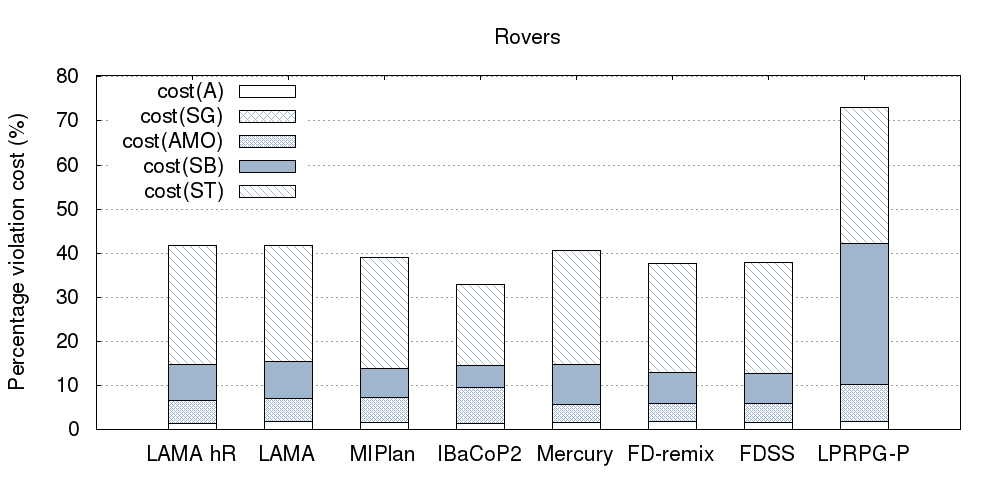
\includegraphics[width=8.5cm]{histogrammi/rovers.png}
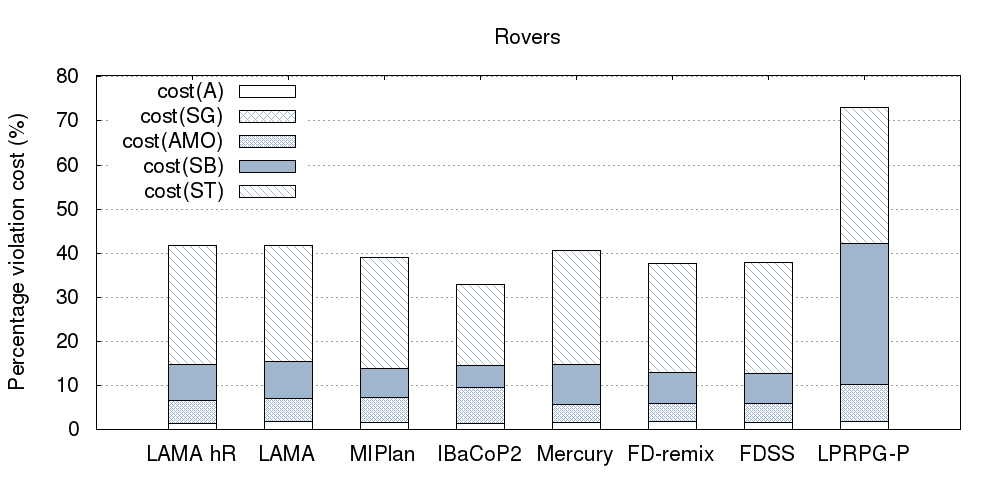
\includegraphics[width=8.5cm]{histogrammi/rovers.png}
\caption{$\alpha_{\text{cost}}$ comparison for Rovers domain.}
\label{hrovers}
\end{figure}

\begin{figure}[]
\centering
% 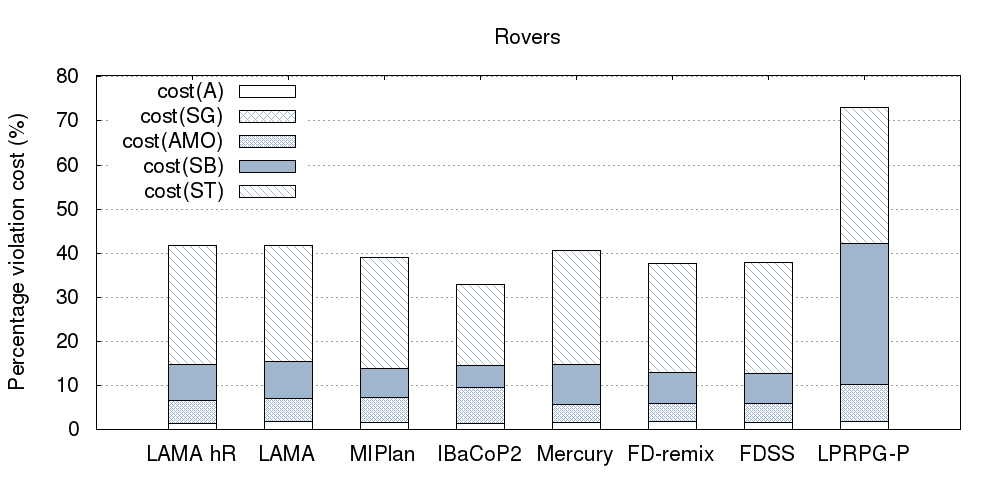
\includegraphics[width=8.5cm]{histogrammi/rovers.png}
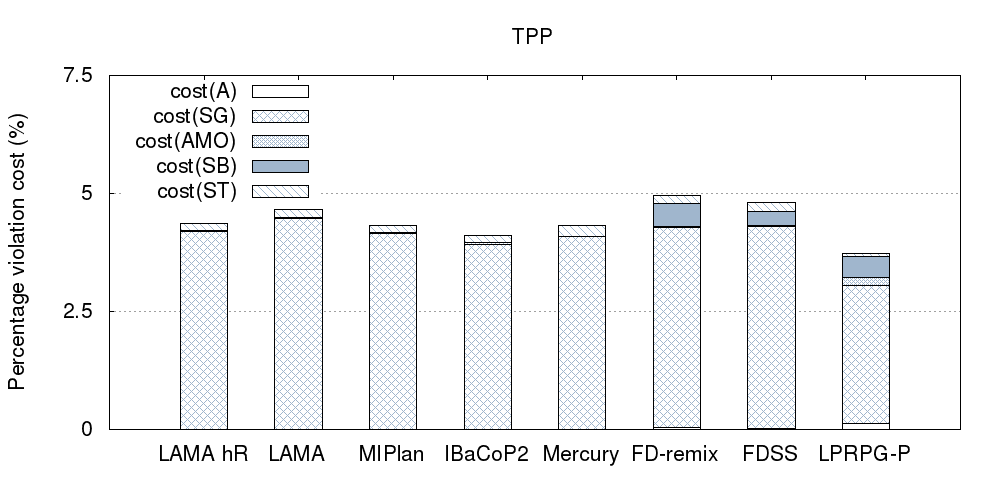
\includegraphics[width=8.5cm]{histogrammi/tpp.png}
\caption{$\alpha_{\text{cost}}$ comparison for TPP domain.}
\label{htpp}
\end{figure}

\begin{figure}[]
\centering
% 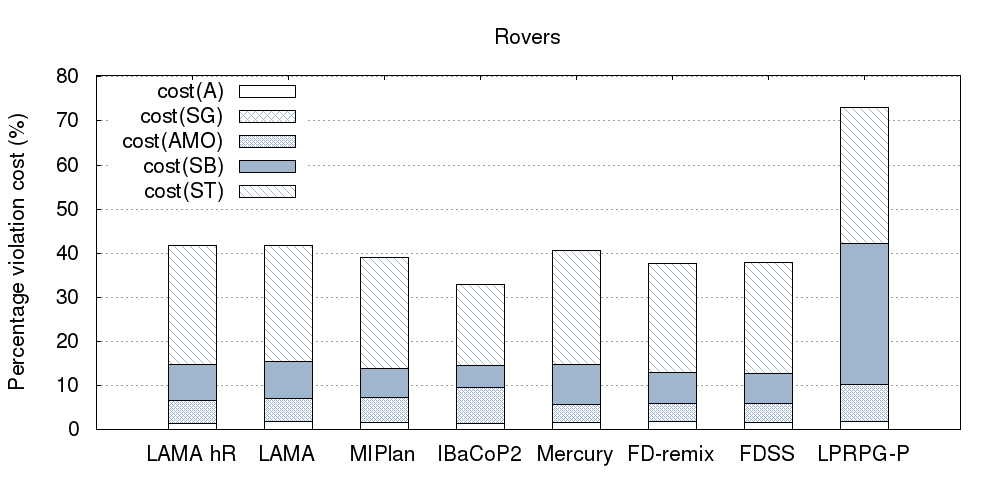
\includegraphics[width=8.5cm]{histogrammi/rovers.png}
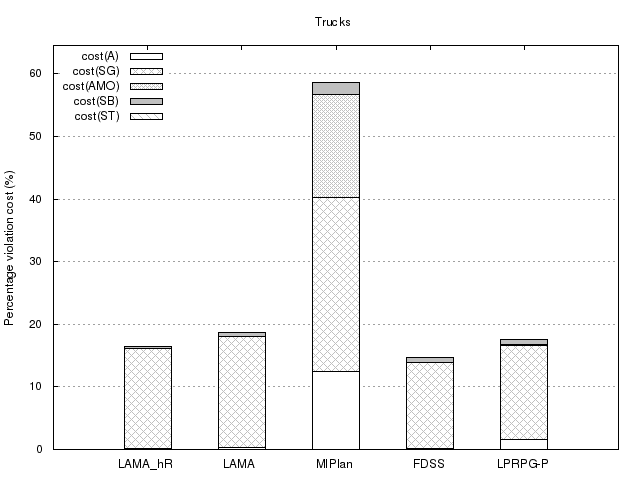
\includegraphics[width=8.5cm]{histogrammi/trucks.png}
\caption{$\alpha_{\text{cost}}$ comparison for Trucks domain.}
\label{htrucks}
\end{figure}

\begin{figure}[]
\centering
% 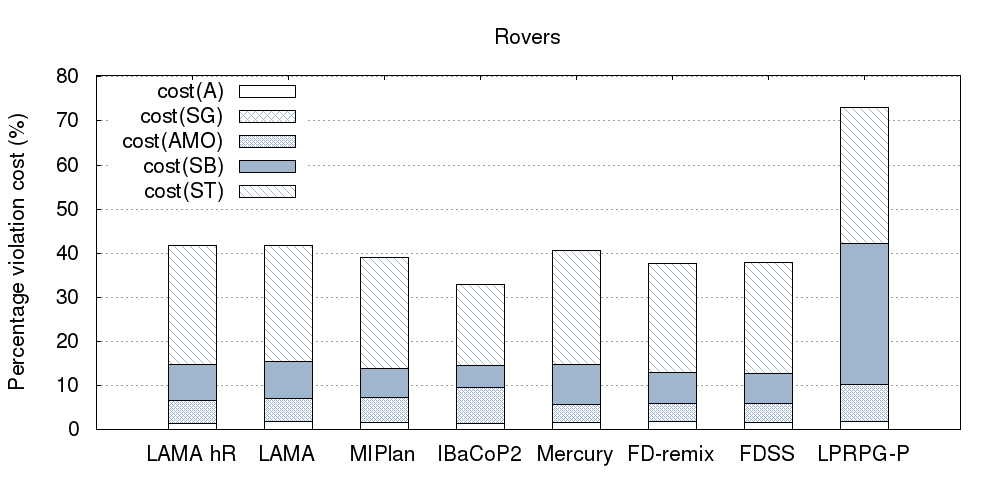
\includegraphics[width=8.5cm]{histogrammi/rovers.png}
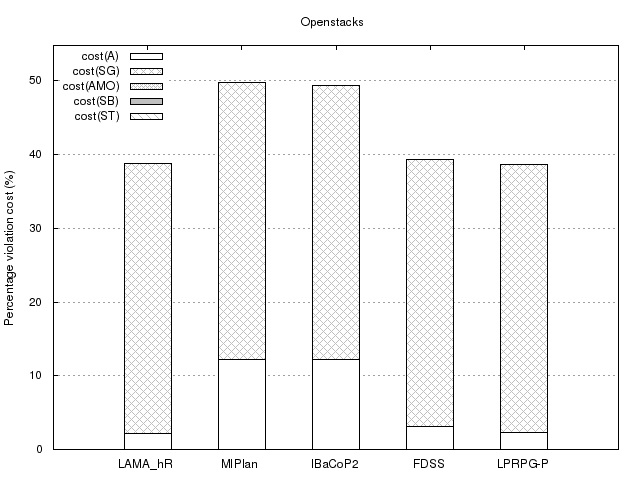
\includegraphics[width=8.5cm]{histogrammi/openstacks.png}
\caption{$\alpha_{\text{cost}}$ comparison for Openstacks domain.}
\label{hopenstacks}
\end{figure}

\begin{figure}[]
\centering
% 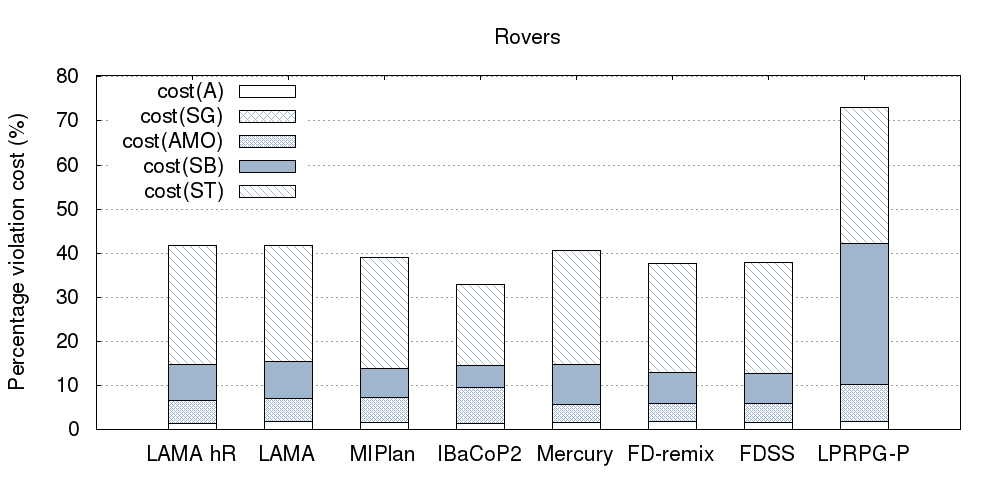
\includegraphics[width=8.5cm]{histogrammi/rovers.png}
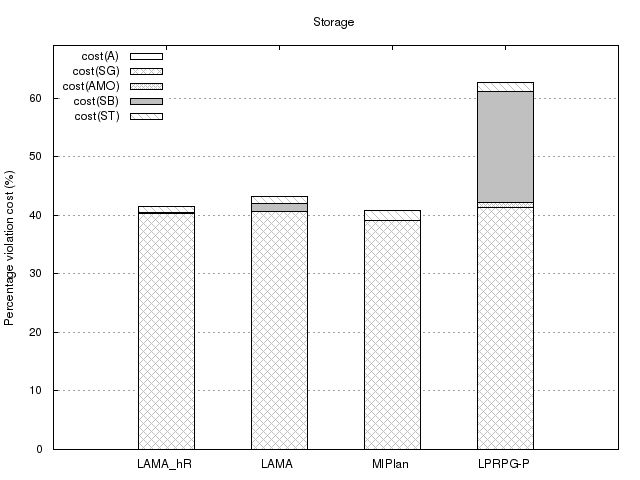
\includegraphics[width=8.5cm]{histogrammi/preprocessed-storage.png}
\caption{$\alpha_{\text{cost}}$ comparison for Storage domain.}
\label{hstorage}
\end{figure}




\subsection{Optimal Planning Results}

\begin{table}[]
\scriptsize
\centering
\begin{tabular}{|c||c|c||c|c||c|c||}
\hline 
\multirow{2}{*}{Domain} & \multicolumn{2}{c||}{$h^{\text{blind}}$} & \multicolumn{2}{c||}{$h^{\text{max}}$} & \multicolumn{2}{c||}{$h^{\text{cpdb}}$} \\ \cline{2-7}
& WRB & PG & WRB & PG & WRB & PG \\ \hline
Storage & 24.78 & {\bf 57.0} & 29.2 & {\bf45.0} & 23.10 & 57.0 \\ \hline
Rovers & 17.4 & {\bf24.0} & 21.43 & {\bf 25.0} & 15.17 & 23.0 \\ \hline
Trucks & 18.84 & {\bf24.0} & 23.19 & 25.0 & n/a & 25 \\ \hline
TPP & --- & 47.0 & --- & 45.0 & -- & 40.0 \\ \hline
\end{tabular}
\caption{Coverage of our (PG) and Nebel compilation scheme (WRB) on the IPC5 benchmarks set with
additional instances with random sampled soft-trajectory constraints, A*
search for optimal solution. Our results concerning the sampled instances are averaged 
for each generated instance. The best performance are indicated in bold.}
\label{coverage_admissible_heuristics}
\end{table}

% STESSA TABELLA MA CON HEURISTICA M&S
% \begin{table}[]
% \scriptsize
% \centering
% \begin{tabular}{|c||c|c||c|c||c|c||c|c||}
% \hline 
% \multirow{2}{*}{DOMINO} & \multicolumn{2}{c||}{$h^{\text{blind}}$} & \multicolumn{2}{c||}{$h^{\text{max}}$} & \multicolumn{2}{c||}{$h^{\text{m\&s}}$} & \multicolumn{2}{c||}{$h^{\text{cpdb}}$} \\ \cline{2-9}
% & WRB & Our & WRB & Our& WRB & Our& WRB & Our \\ \hline
% Storage & 24.78 & 57.0 & 29.2 & 45.0 & 32.50 & 24.0 & 23.10 & 57.0 \\ \hline
% Rovers & 17.4 & 24.0 & 21.43 & 25.0 & 16.67 & 26.0 & 15.17 & 23.0 \\ \hline
% Trucks & 18.84 & 24.0 & 23.19 & 25.0 & n/a & 25.0 & n/a & 25 \\ \hline
% TPP & --- & 47.0 & --- & 45.0 & --- & 47.0 & -- & 40.0 \\ \hline
% \end{tabular}
% \caption{Coverage of our and Nebel compilation scheme on the IPC5 benchmarks set with
% additional instances with random sampled soft-trajectory constraints, A*
% search for optimal solution. Our results concerning the sampled instances are averaged. The best performance are indicated in bold.}
% \label{coverage_admissible_heuristics}
% \end{table}


\section{Conclusions}



\bibliographystyle{plain}
\bibliography{biblio.bib}
\end{document}
